% Auto-generated manuscript asset skeleton for TGRS VCEA / SS-VCEA writing
% Generated on 2026-05-14

\section*{Draft Figure and Table Floats}
\noindent This file collects the current figure/table draft captions, labels, and source paths for the manuscript asset package.

% Recommended packages:
% \usepackage{graphicx}
% \usepackage{booktabs}
% \usepackage{adjustbox}
% \usepackage{threeparttable}
% \usepackage{float}
% \usepackage{url}

\subsection*{Figures}

\begin{figure*}[t]
  \centering
  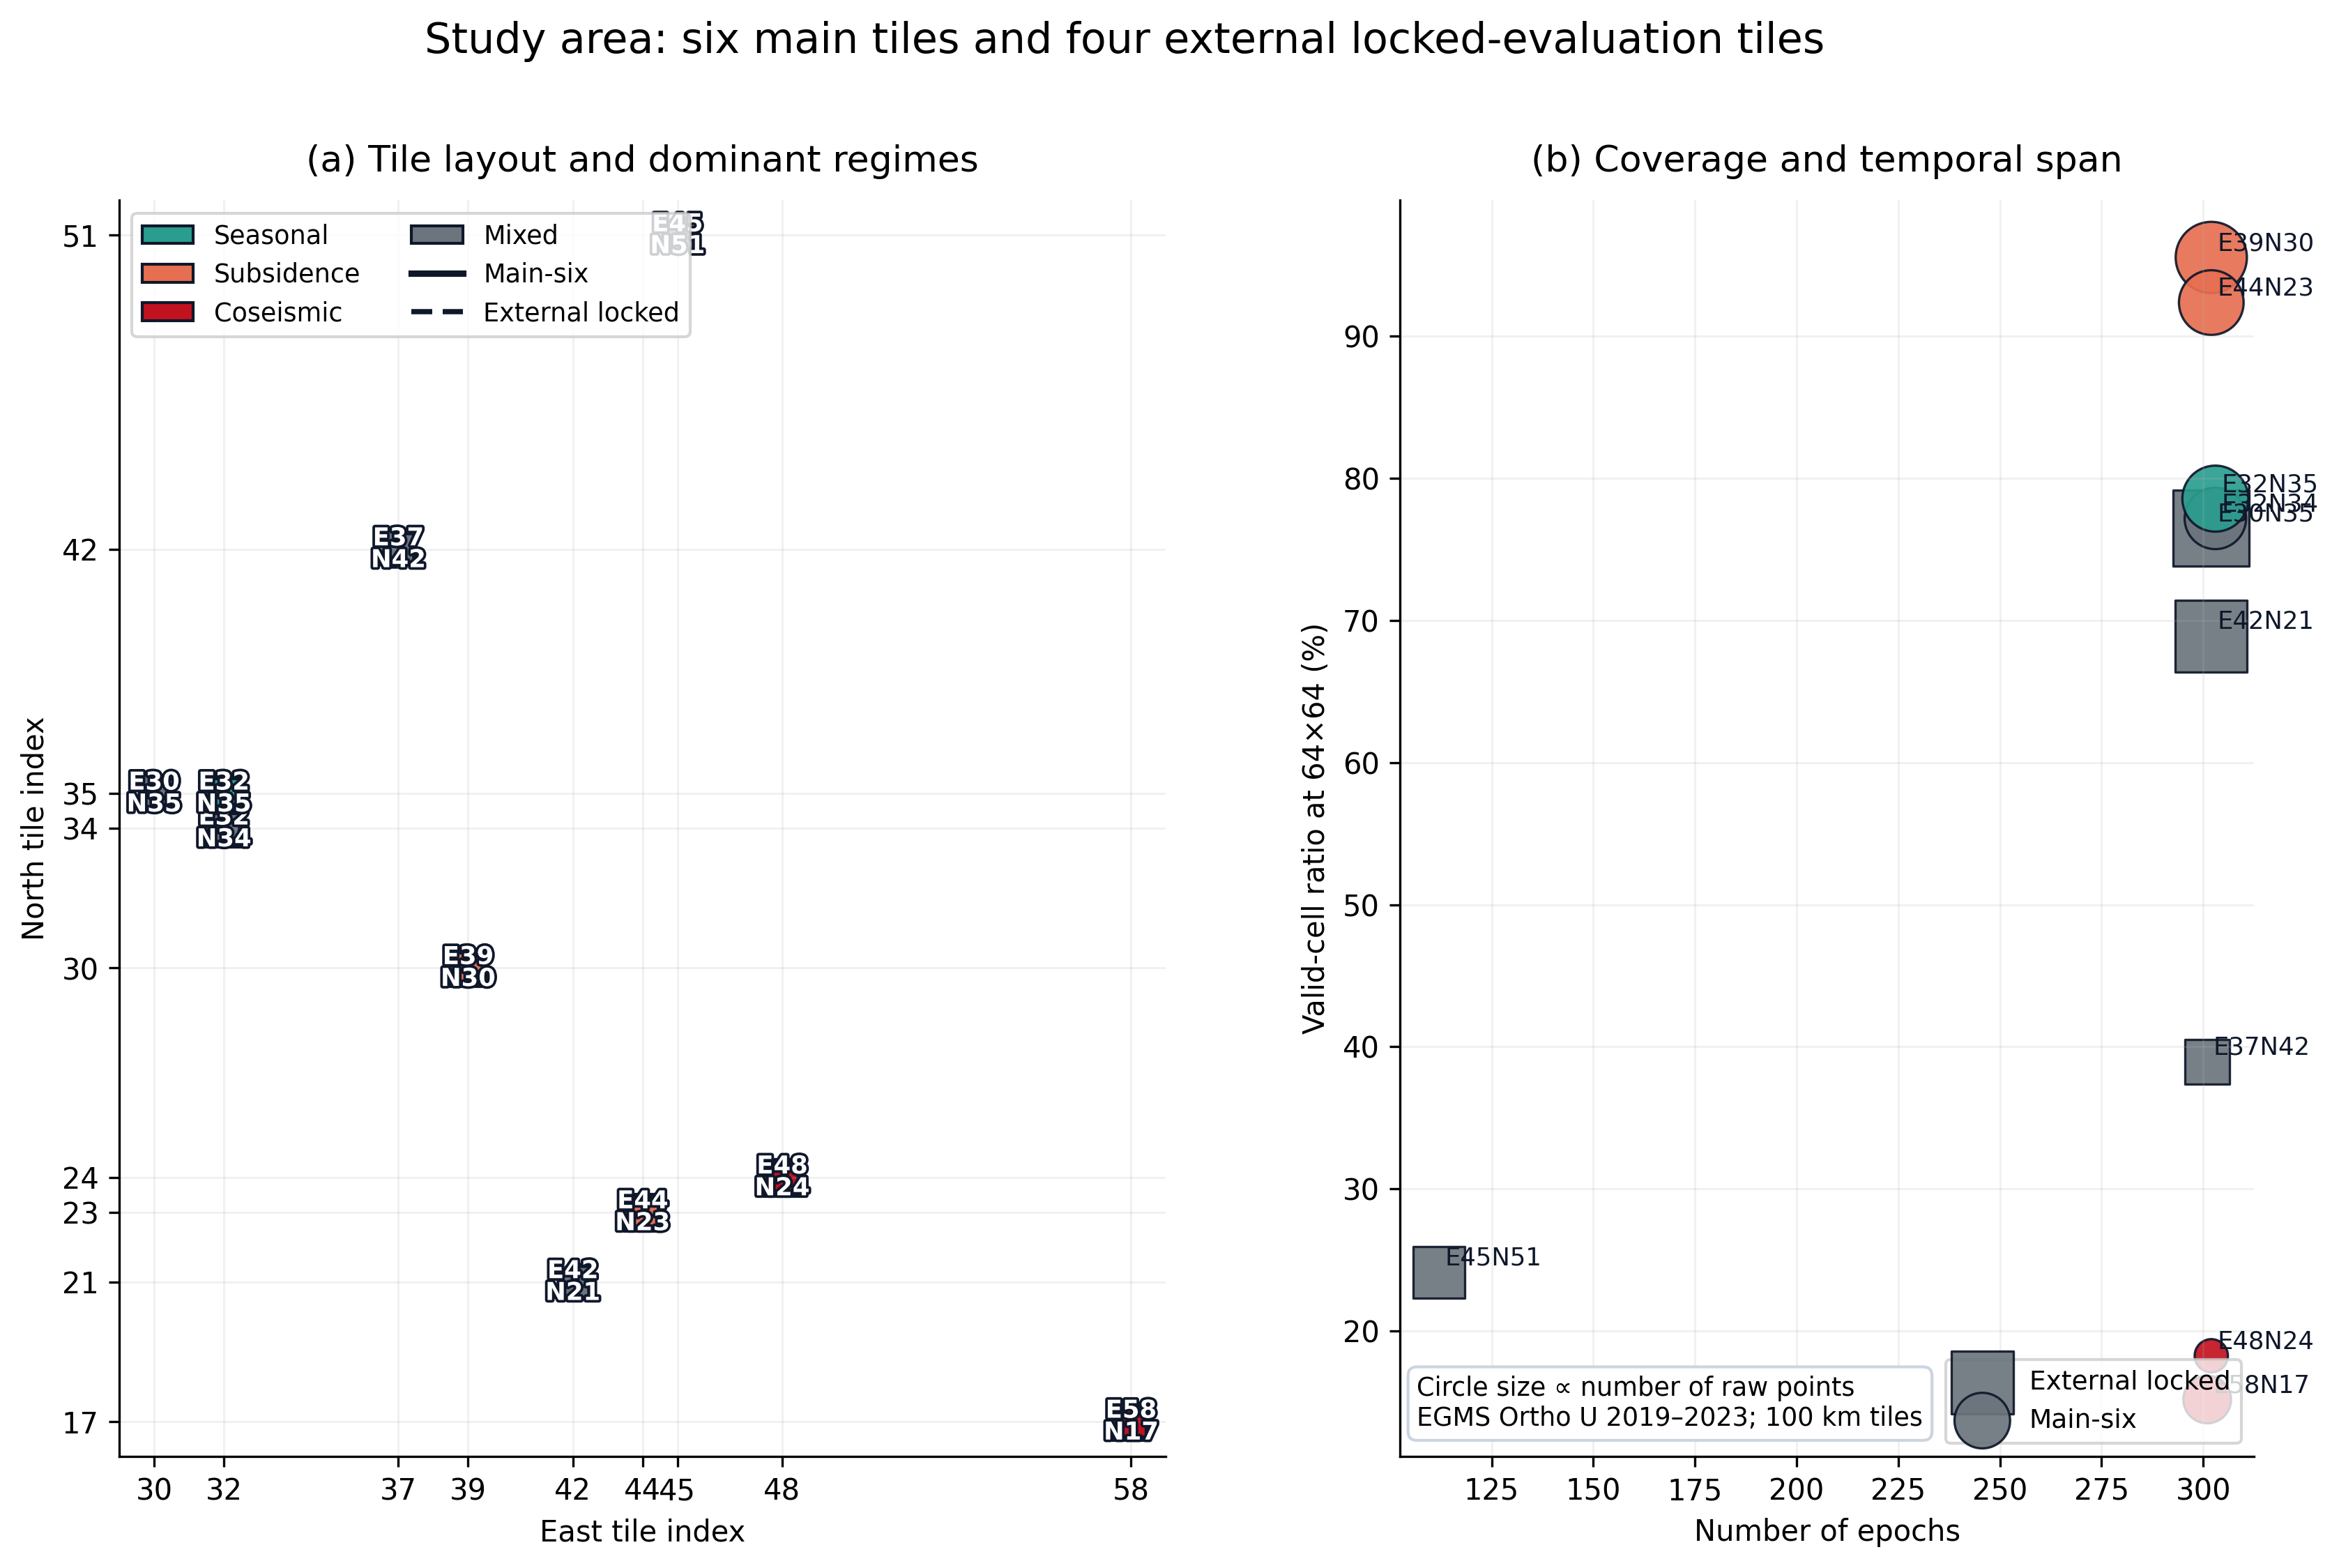
\includegraphics[width=0.98\textwidth]{figures/final/Fig01_study_area_map.png}
  \caption{Study area and coverage of the unified EGMS 2019--2023 Ortho U benchmark. (a) The six main-development tiles and four external locked-evaluation tiles are shown with their dominant regime labels. (b) Temporal span and valid-cell coverage at the primary $64\times64$ setting. Main-six tiles were used for model development, whereas the external four tiles remained frozen for locked evaluation.}
  \label{fig:fig01}
\end{figure*}

\begin{figure*}[t]
  \centering
  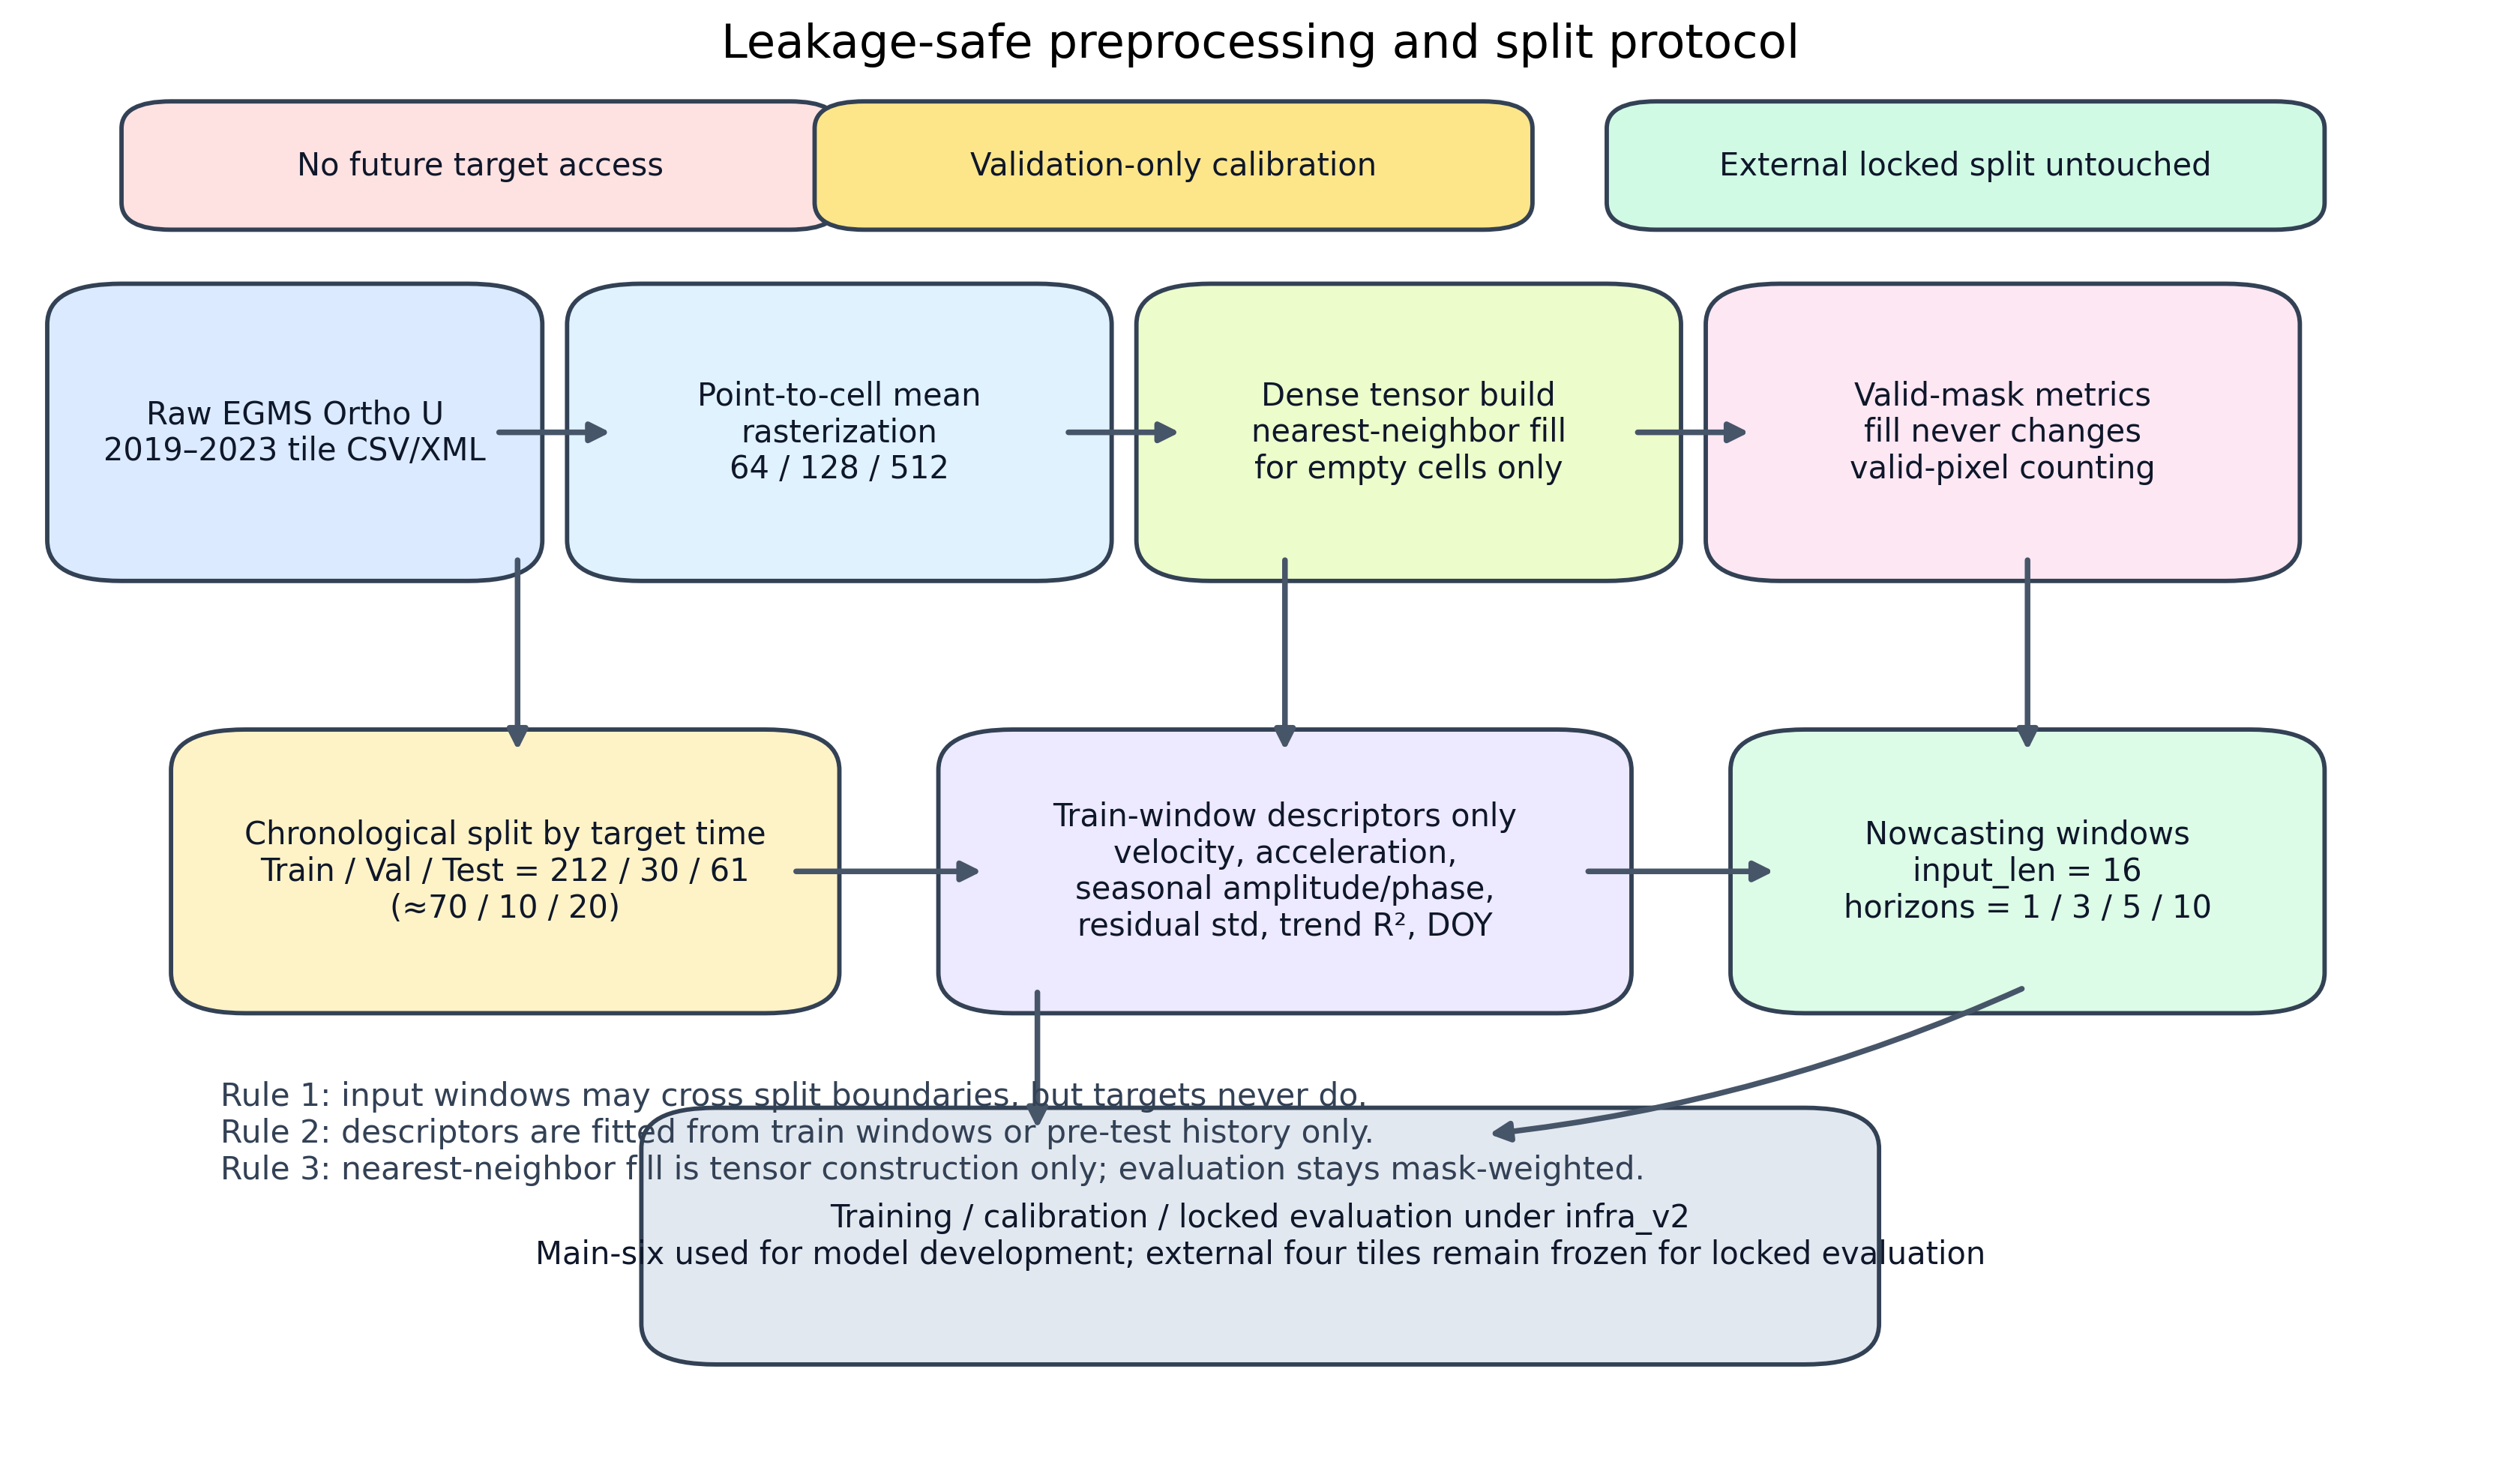
\includegraphics[width=0.98\textwidth]{figures/final/Fig02_leakage_safe_pipeline.png}
  \caption{Leakage-safe preprocessing and split protocol. Raw EGMS point observations were rasterized by point-to-cell mean aggregation, converted into dense tensors with nearest-neighbor fill for empty cells only, and evaluated with valid-mask weighted metrics. Chronological train/validation/test splits were assigned by target time, descriptors were computed from train windows or pre-test history only, and the external locked split remained untouched throughout model search.}
  \label{fig:fig02}
\end{figure*}

\begin{figure*}[t]
  \centering
  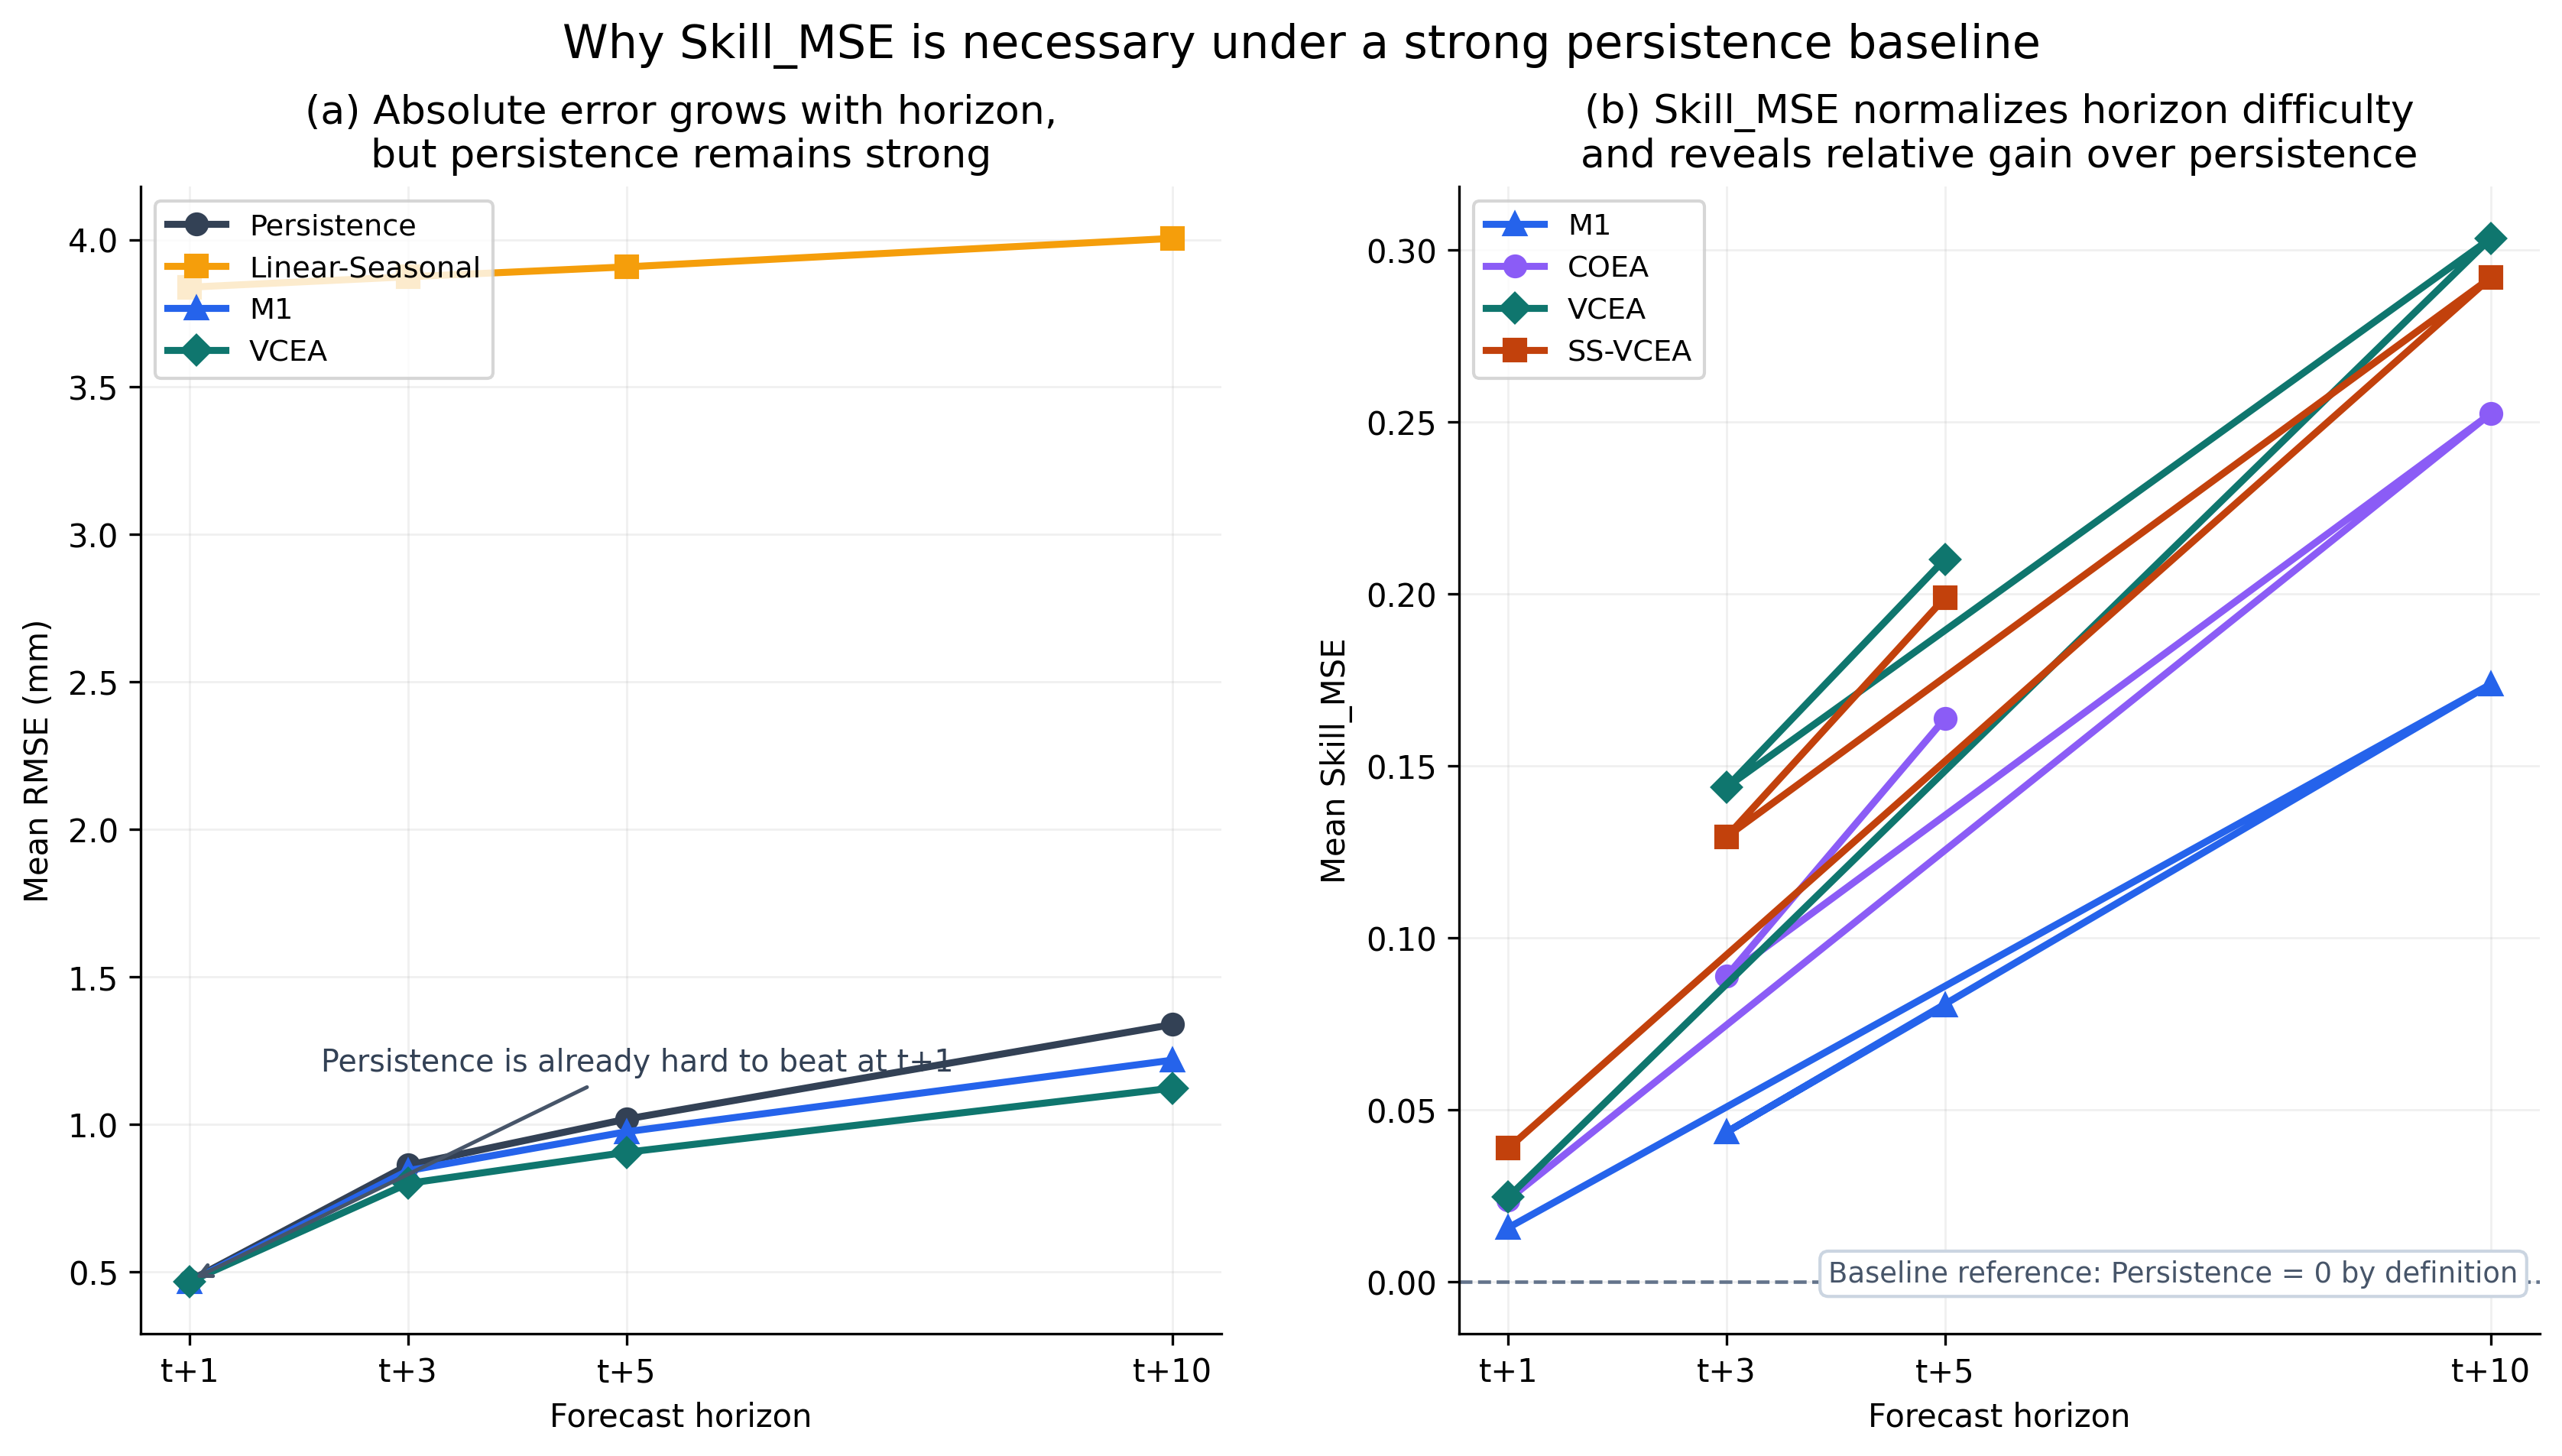
\includegraphics[width=0.98\textwidth]{figures/final/Fig03_persistence_and_horizon_difficulty.png}
  \caption{Why Skill\_MSE is required under a strong persistence baseline. (a) Absolute RMSE grows with horizon, but persistence remains highly competitive, especially at $t{+}1$. (b) Skill\_MSE normalizes horizon difficulty and makes relative gains over persistence directly comparable across horizons and models.}
  \label{fig:fig03}
\end{figure*}

\begin{figure*}[t]
  \centering
  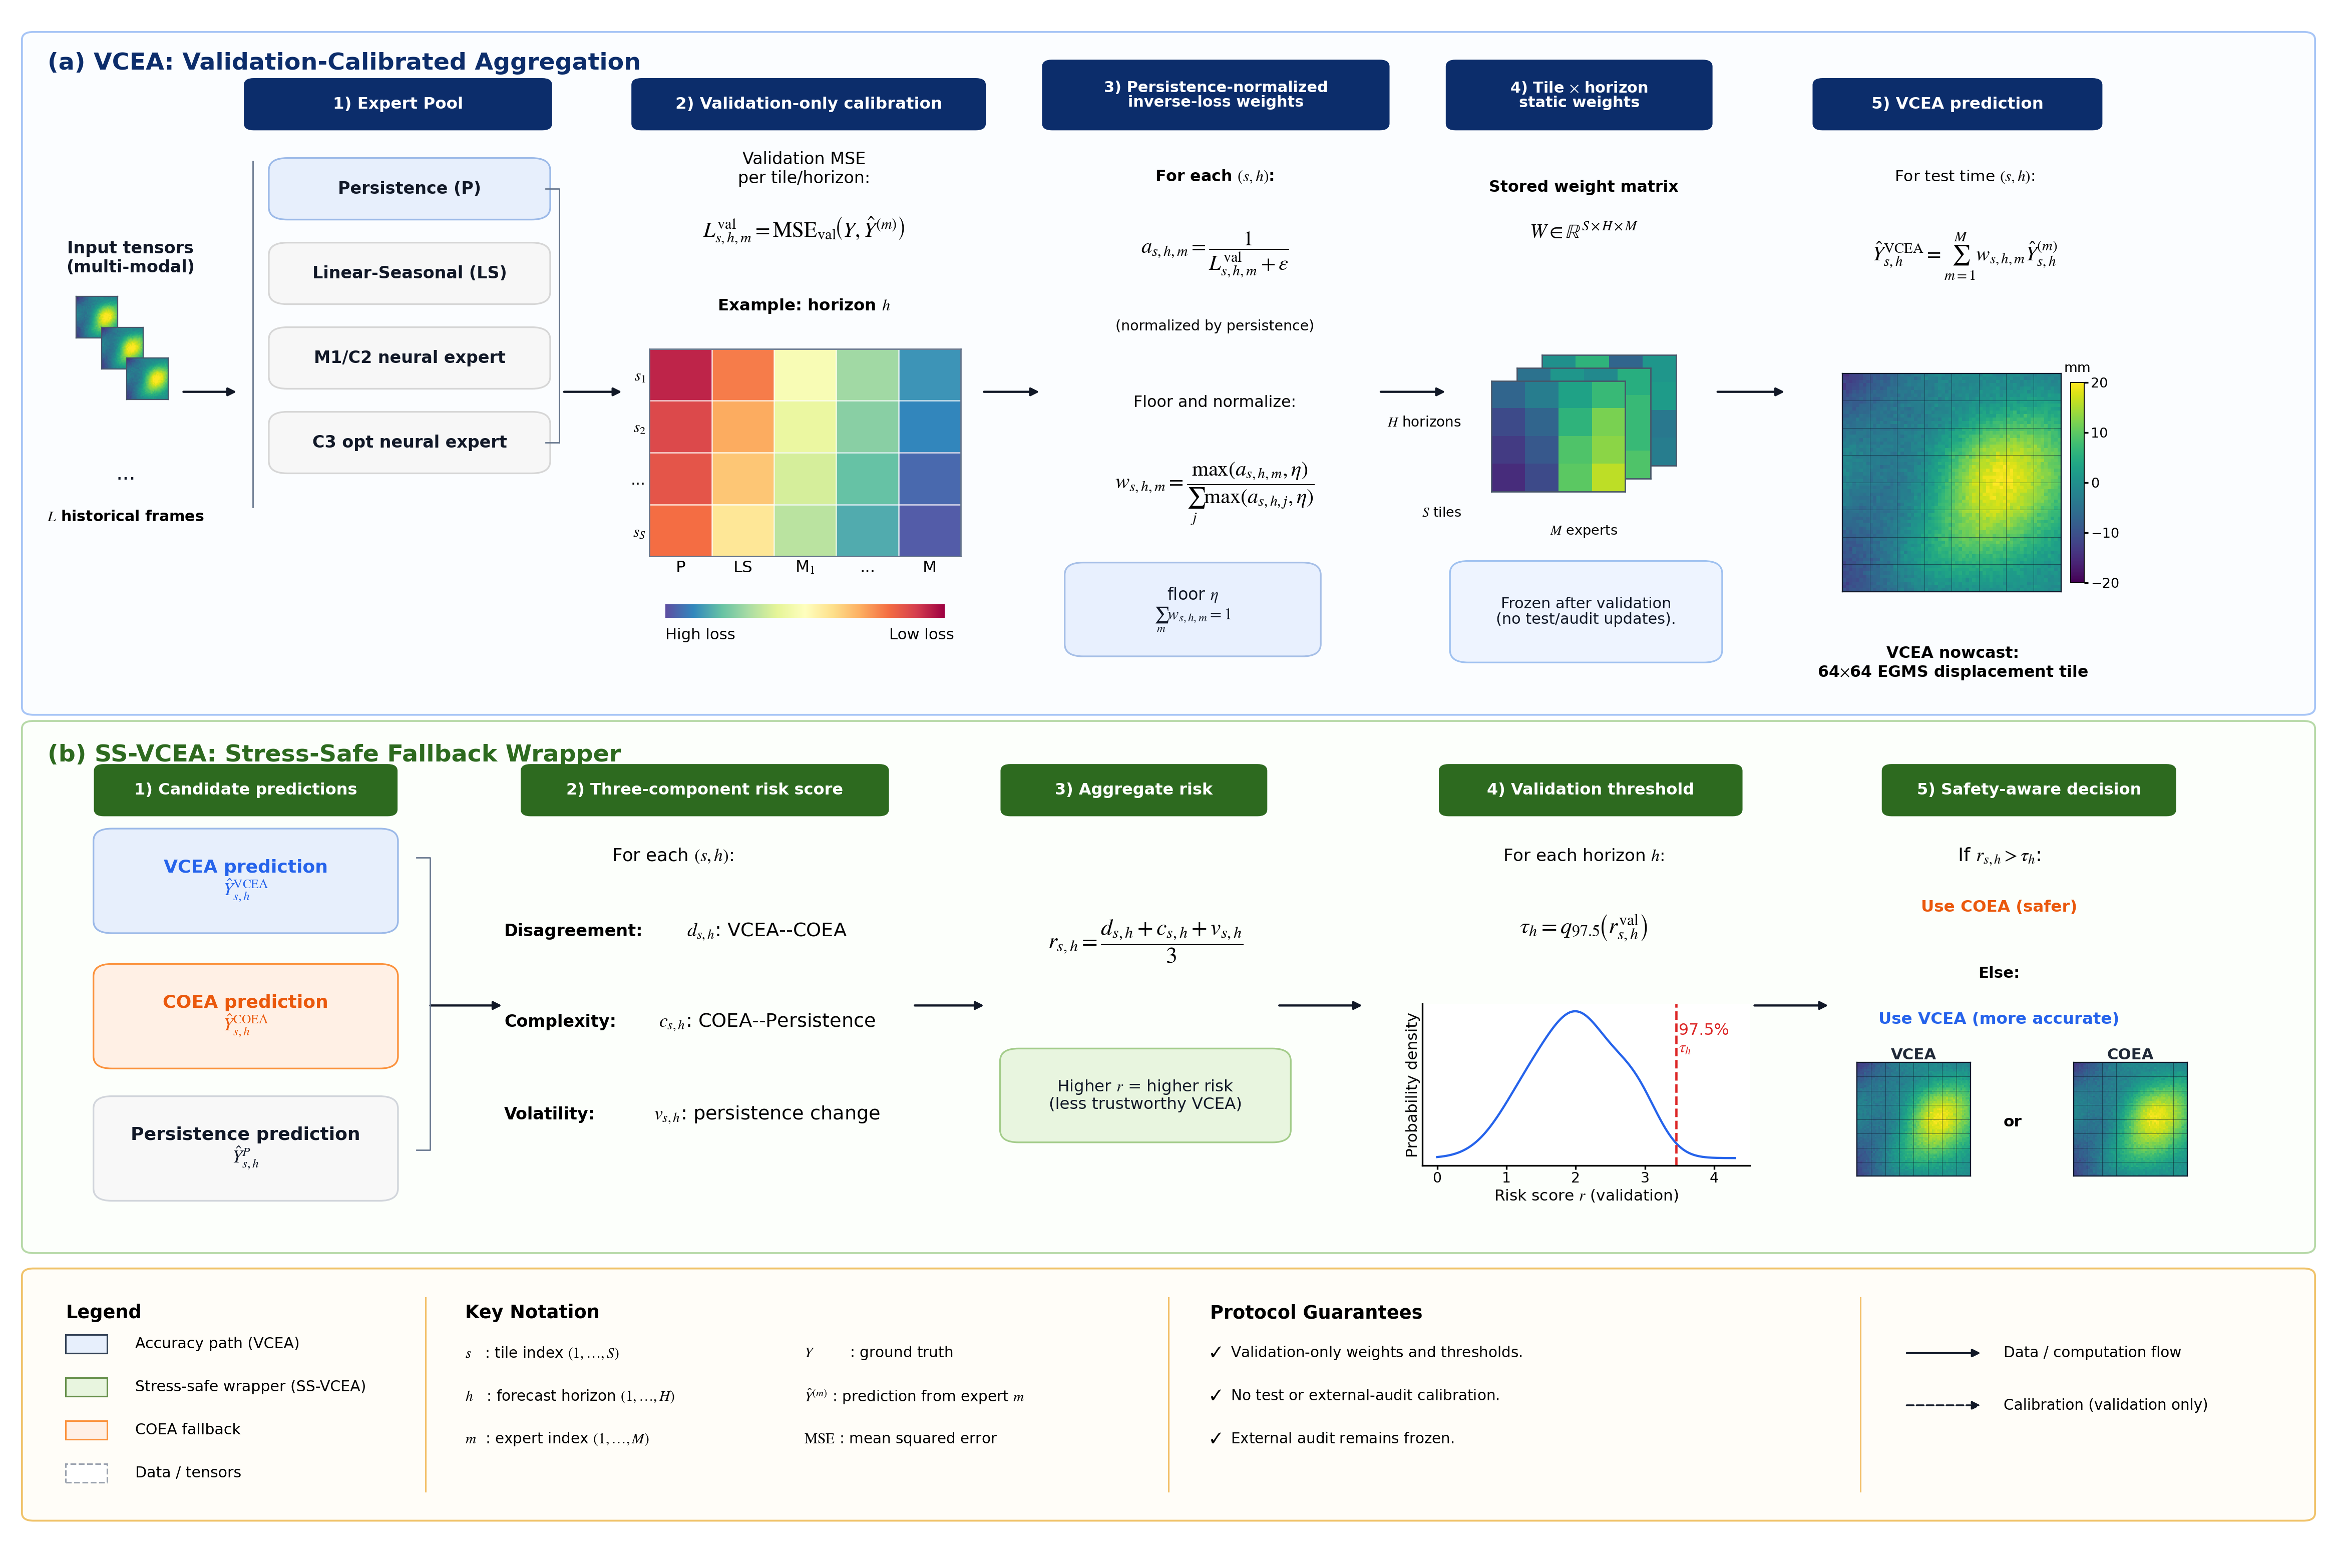
\includegraphics[width=0.98\textwidth]{figures/final/Fig04_vcea_ssvcea_method.png}
  \caption{Method overview of VCEA and SS-VCEA. VCEA performs validation-only static expert calibration over the expert pool $\{\text{Persistence},\text{Linear-Seasonal},\text{M1},\text{C3\_opt}\}$ and produces a tile$\times$horizon-specific weighted prediction. SS-VCEA reuses the same expert pool and applies a validation-calibrated hard fallback when the equal-normalized risk score $r=(d+c+v)/3$ exceeds a horizon-specific threshold.}
  \label{fig:fig04}
\end{figure*}

\begin{figure*}[t]
  \centering
  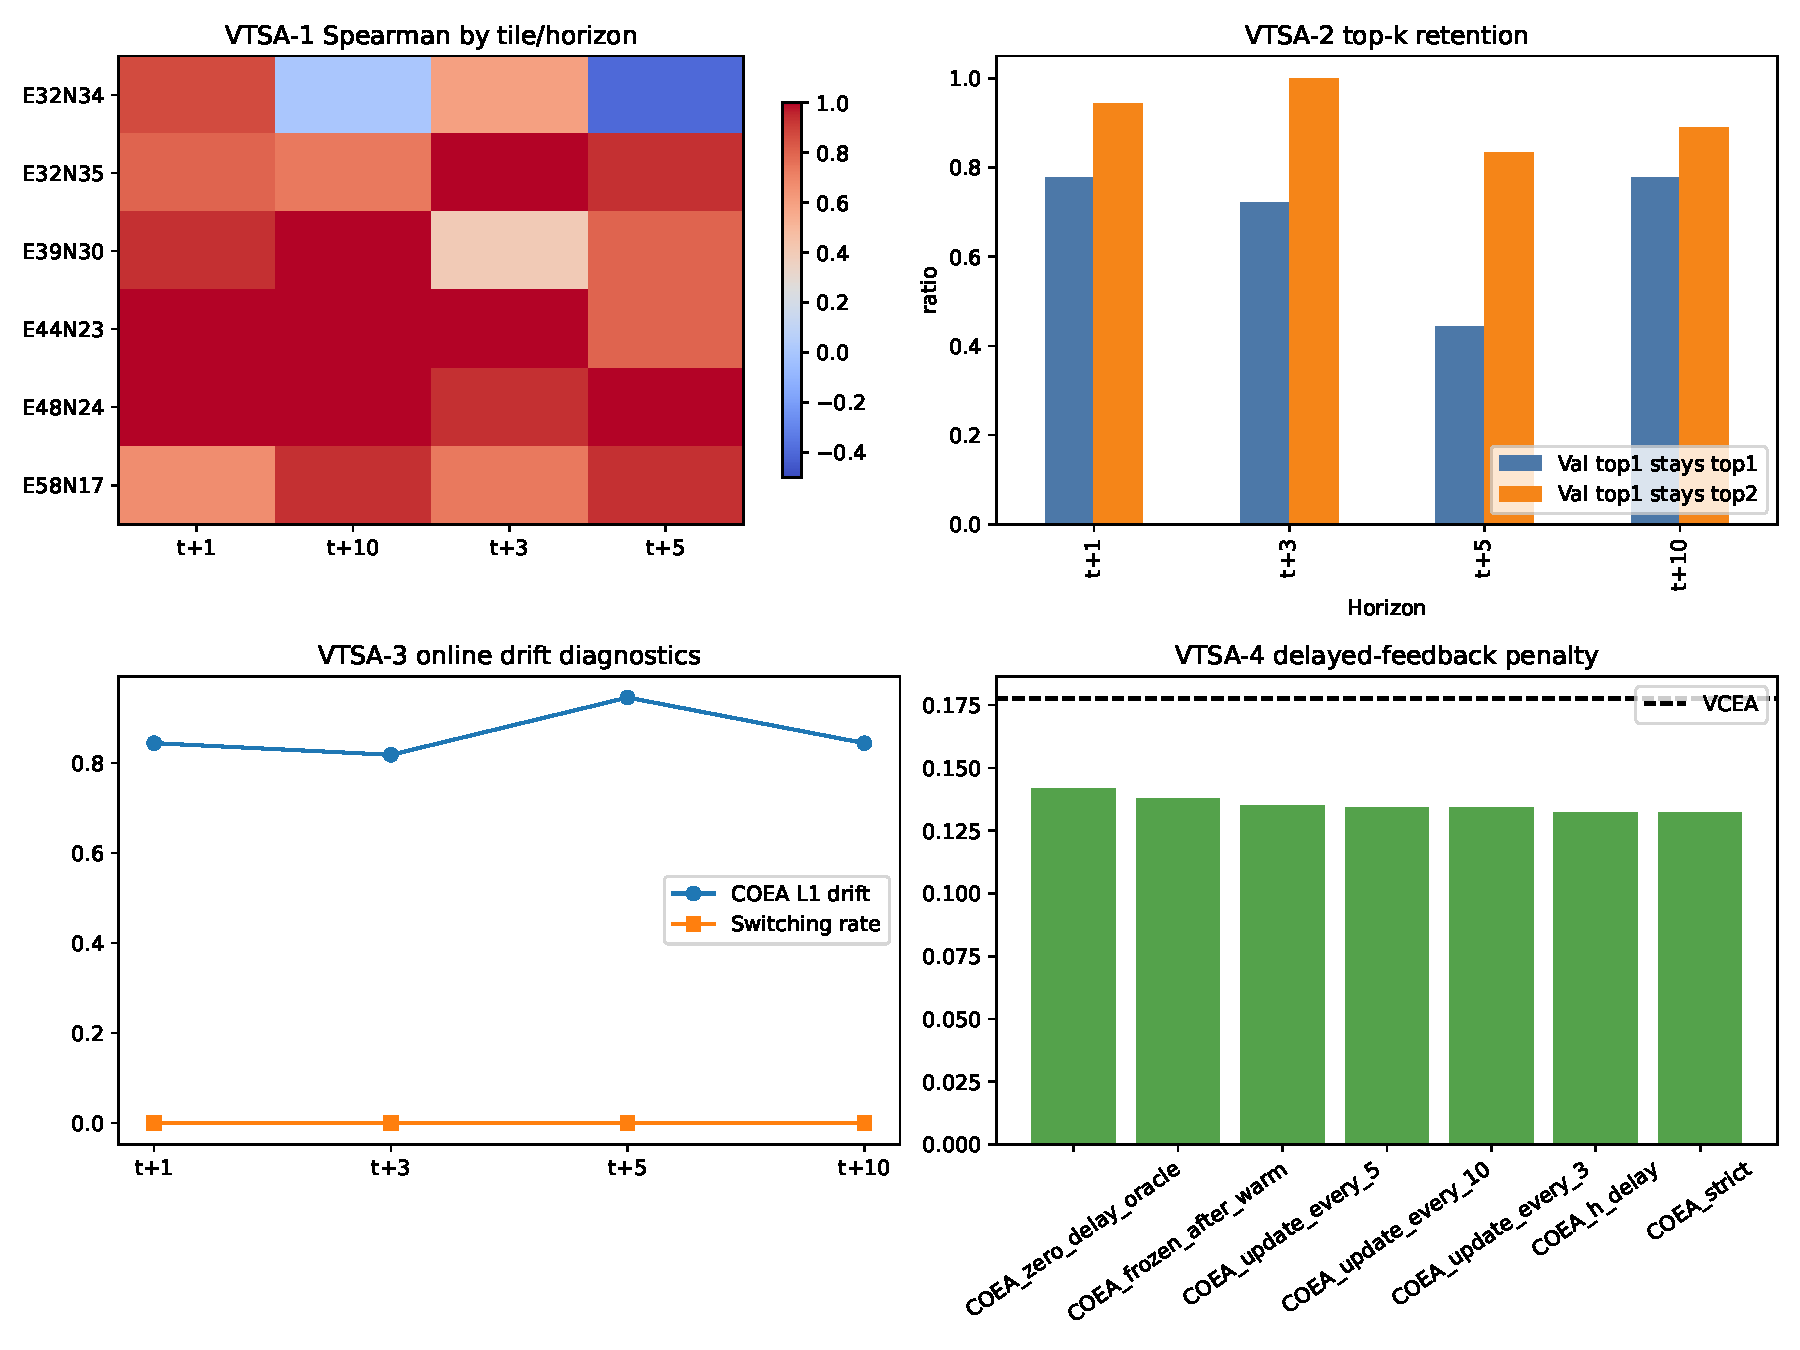
\includegraphics[width=0.98\textwidth]{figures/ready/fig_vtsa_mechanism.pdf}
  \caption{VTSA mechanism evidence. The figure summarizes validation-to-test rank stability, top-$k$ retention, and the drift behavior of online aggregation, providing the mechanism-level explanation for why validation-calibrated static aggregation remains competitive on the test period.}
  \label{fig:fig05}
\end{figure*}

\begin{figure*}[t]
  \centering
  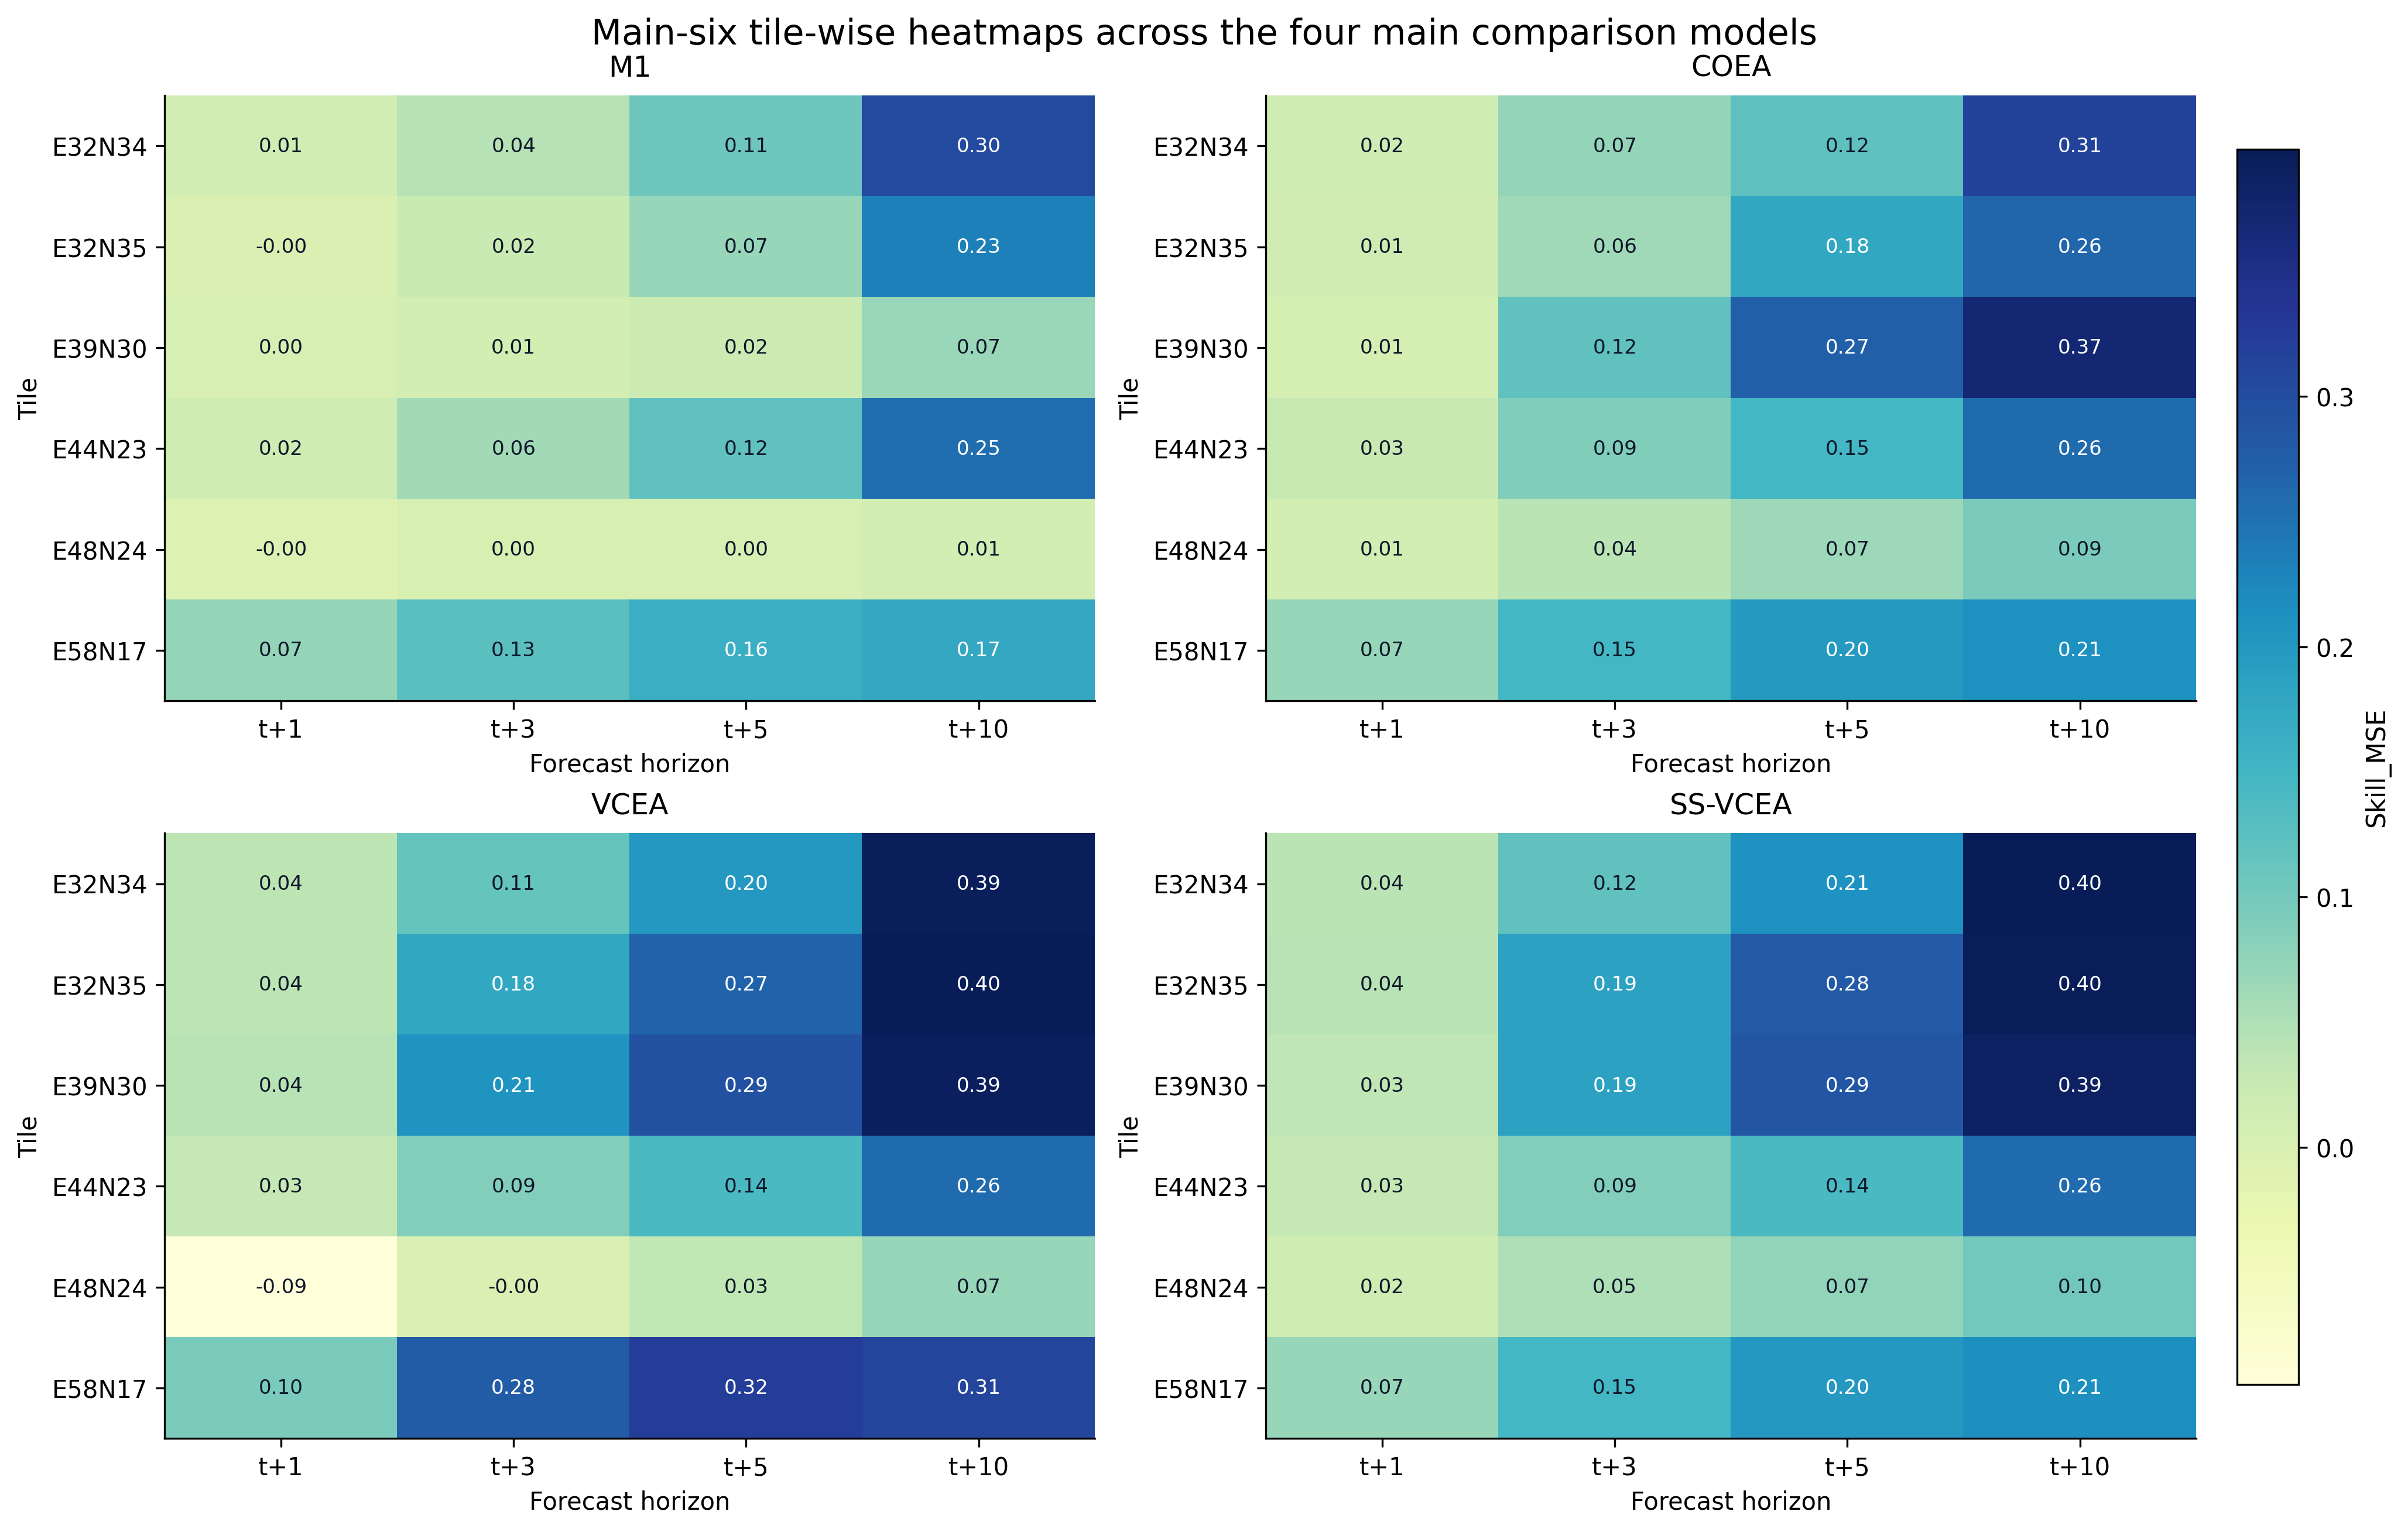
\includegraphics[width=0.98\textwidth]{figures/final/Fig06_main_six_tile_heatmap_panel.png}
  \caption{Main-six tile-wise heatmaps for the four primary comparison models: M1, COEA, VCEA, and the selected SS-VCEA deployment variant. Each cell reports mean Skill\_MSE for one tile-horizon pair. The panel highlights that aggregation gains are spatially heterogeneous, while SS-VCEA largely preserves the tile-wise benefits of VCEA.}
  \label{fig:fig06}
\end{figure*}

\begin{figure*}[t]
  \centering
  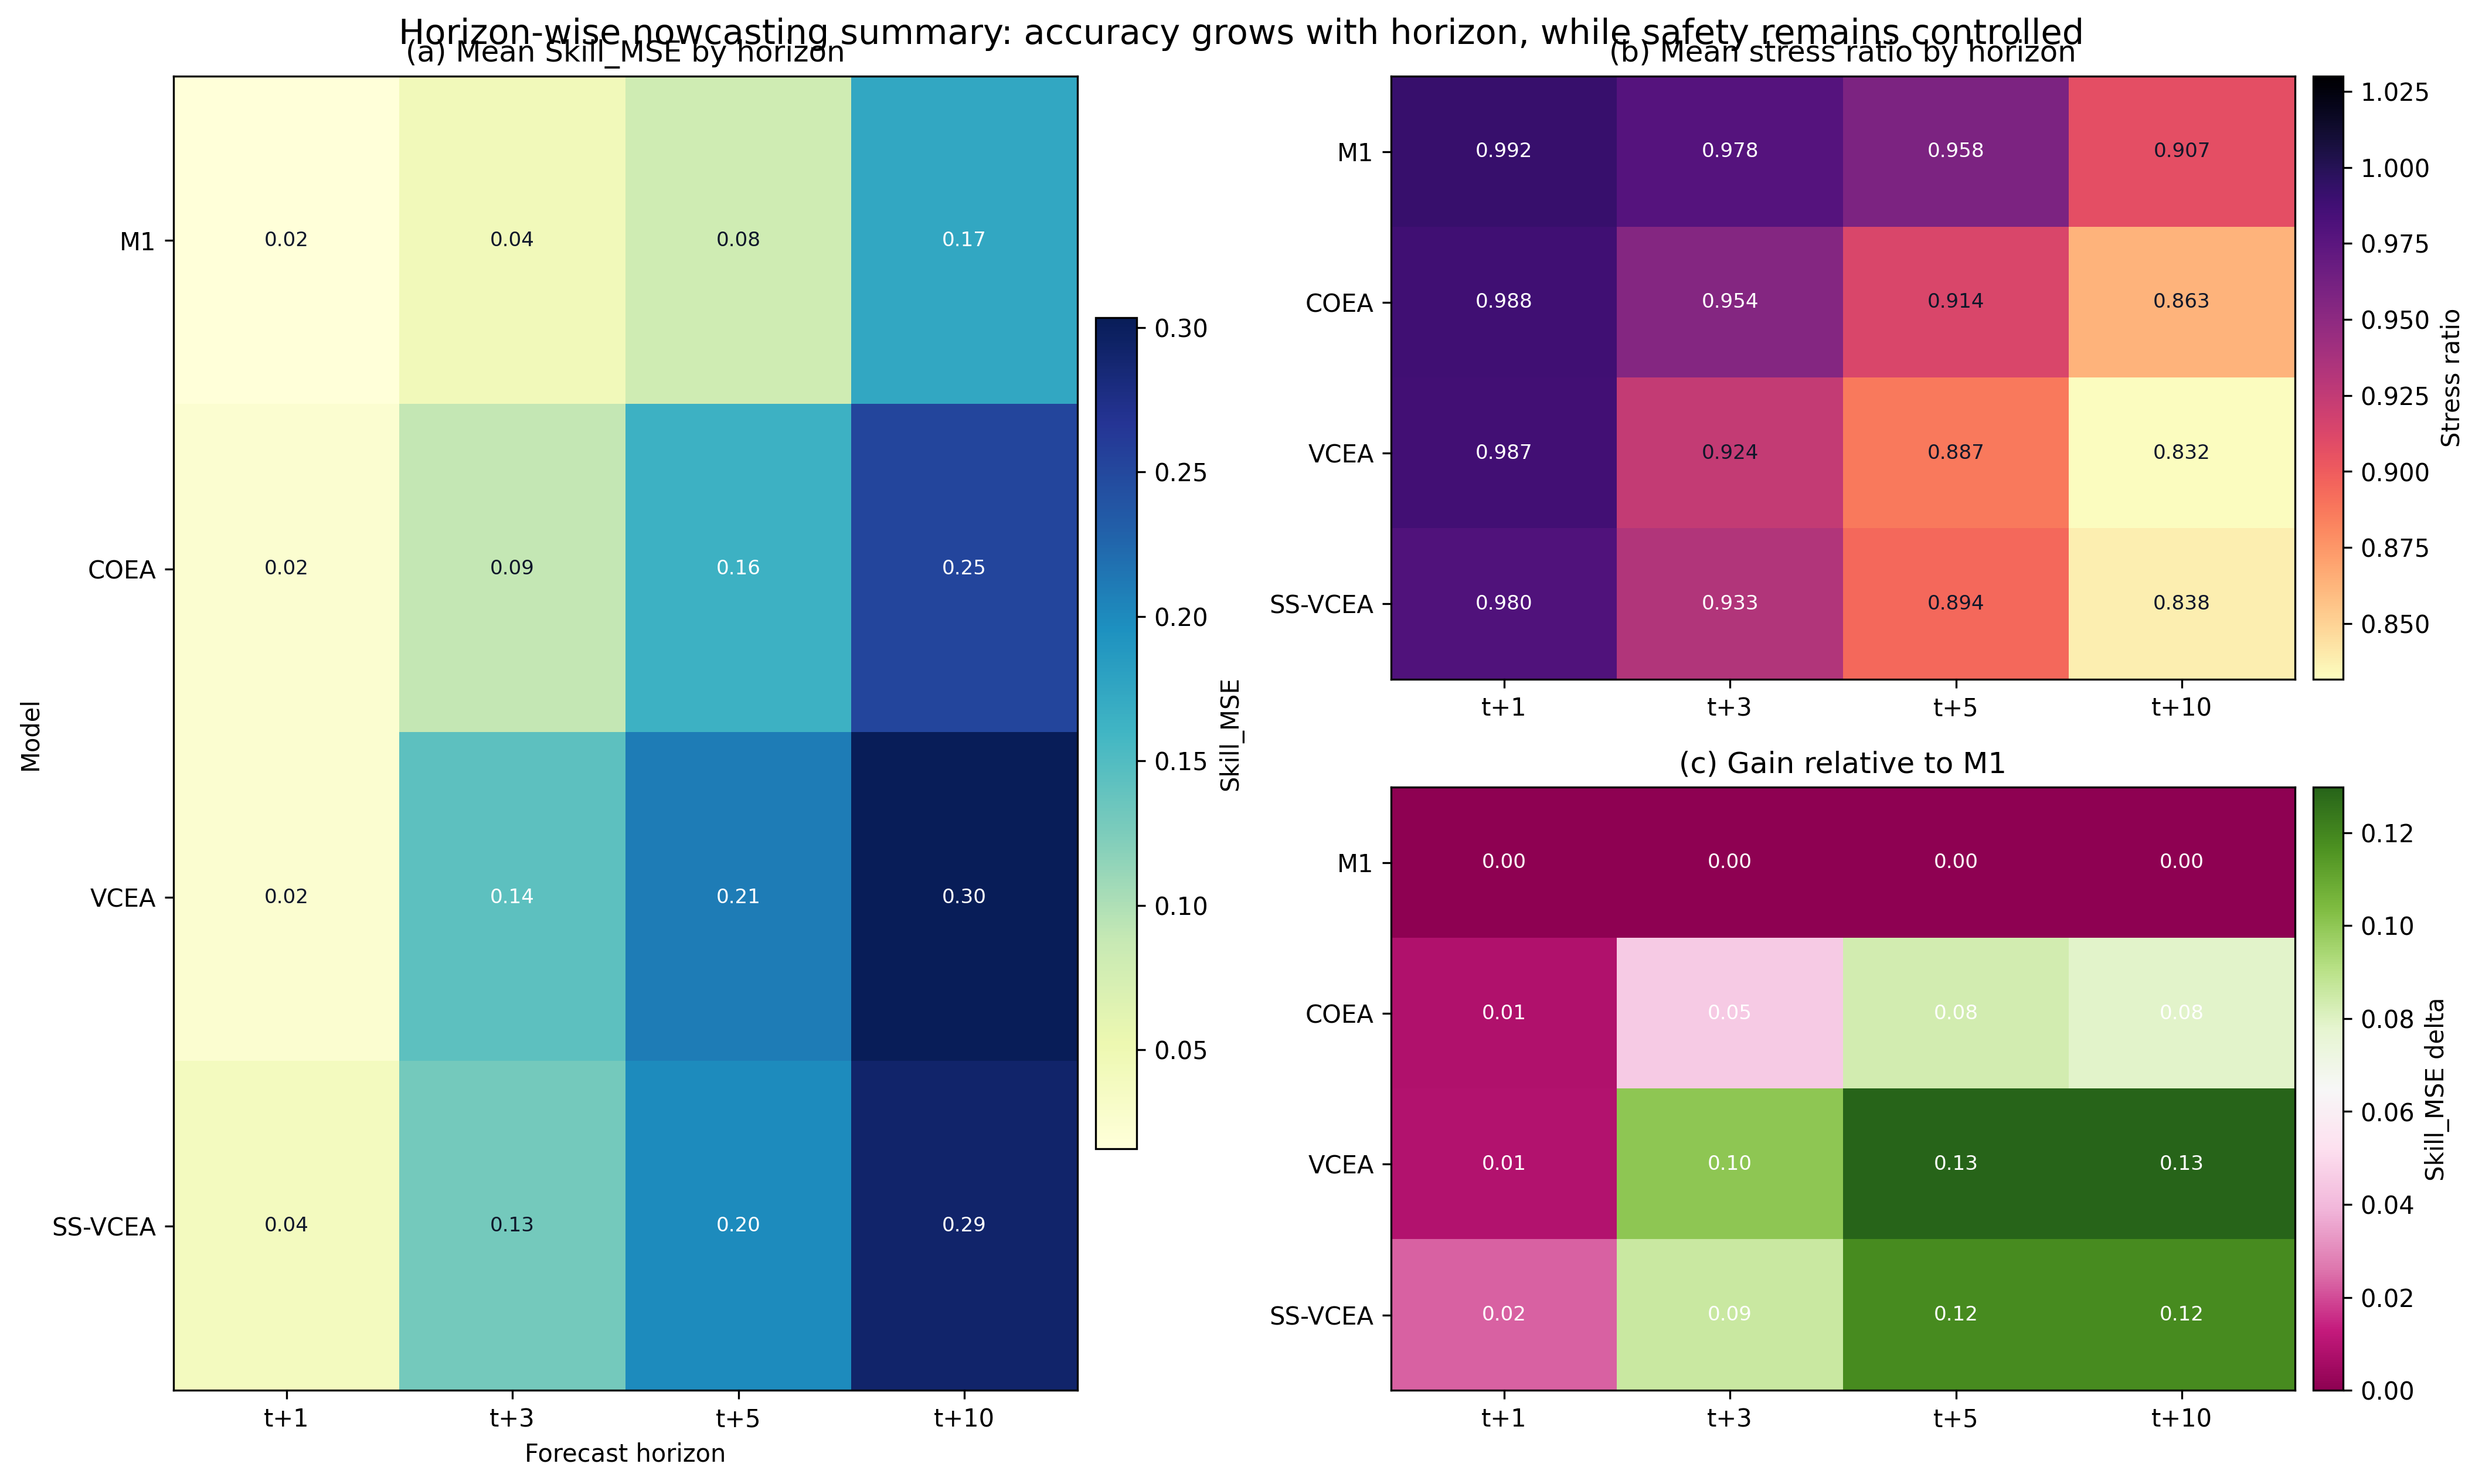
\includegraphics[width=0.98\textwidth]{figures/final/Fig07_horizon_summary_panel.png}
  \caption{Horizon-wise summary of multi-step nowcasting. (a) Mean Skill\_MSE aggregated over the six main tiles. (b) Mean stress ratio by horizon. (c) Mean Skill\_MSE gain relative to M1. The panel shows that aggregation gains increase with horizon, whereas stress remains controlled for COEA and SS-VCEA.}
  \label{fig:fig07}
\end{figure*}

\begin{figure*}[t]
  \centering
  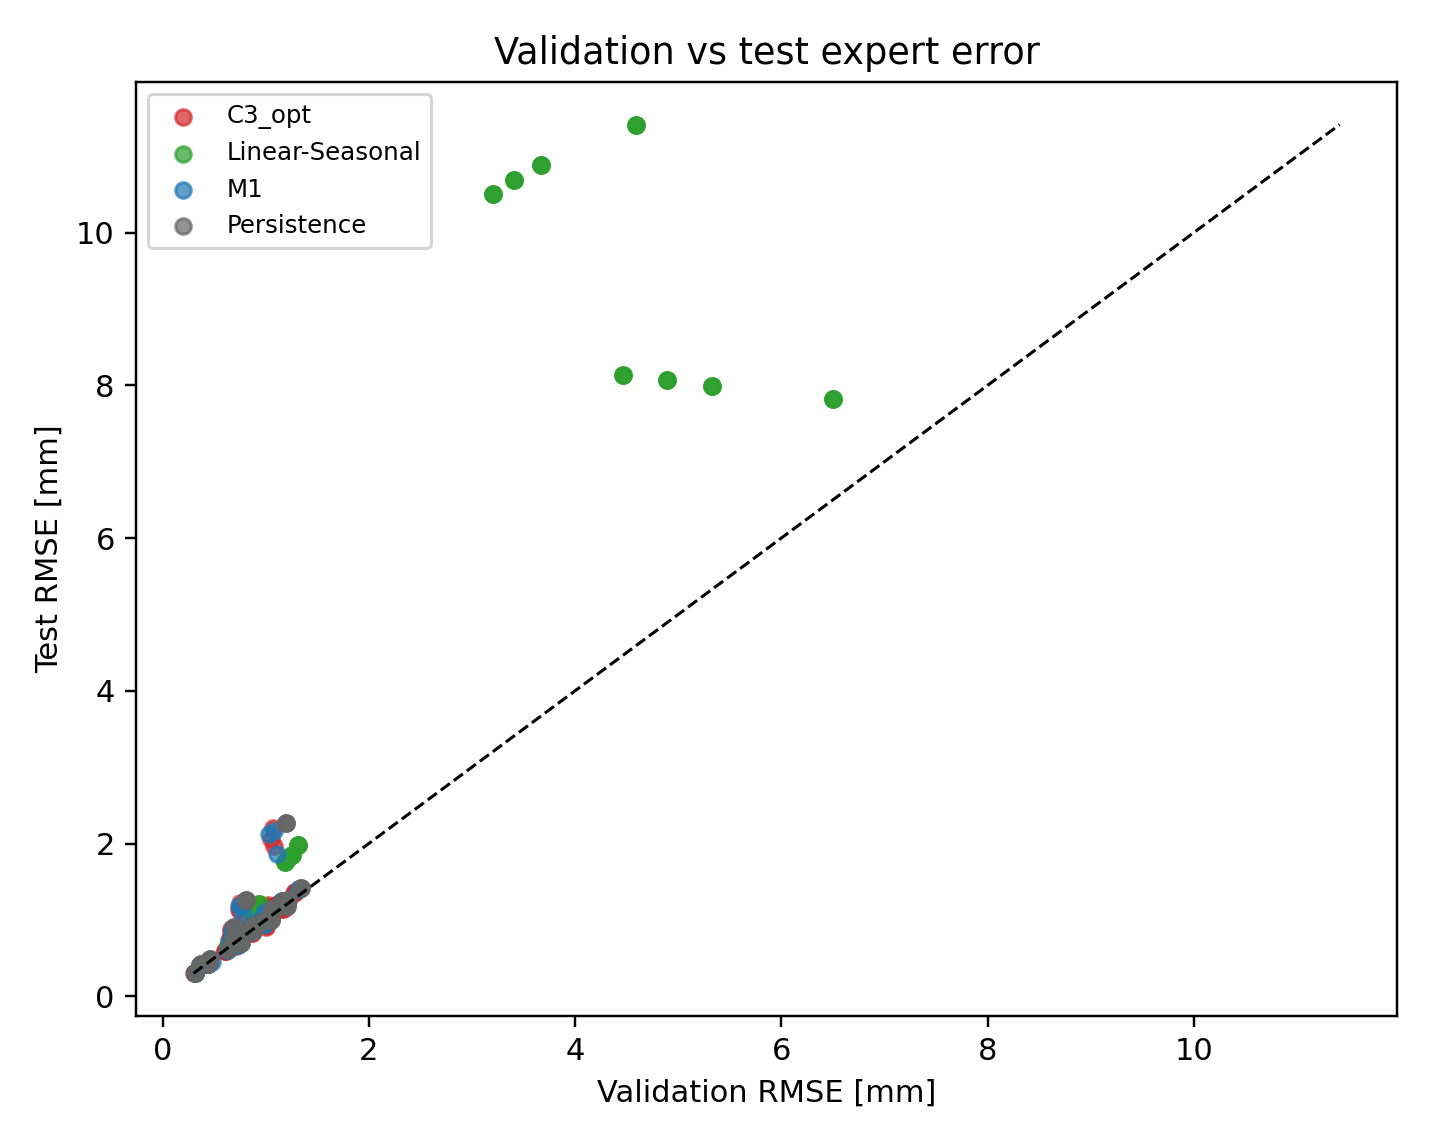
\includegraphics[width=0.98\textwidth]{figures/ready/fig_val_test_rank_scatter.png}
  \caption{Validation ranking versus test ranking for expert performance. The strong validation-to-test agreement supports the use of validation-calibrated static weights in VCEA and helps explain why static aggregation outperforms delayed-feedback online updates.}
  \label{fig:fig08}
\end{figure*}

\begin{figure*}[t]
  \centering
  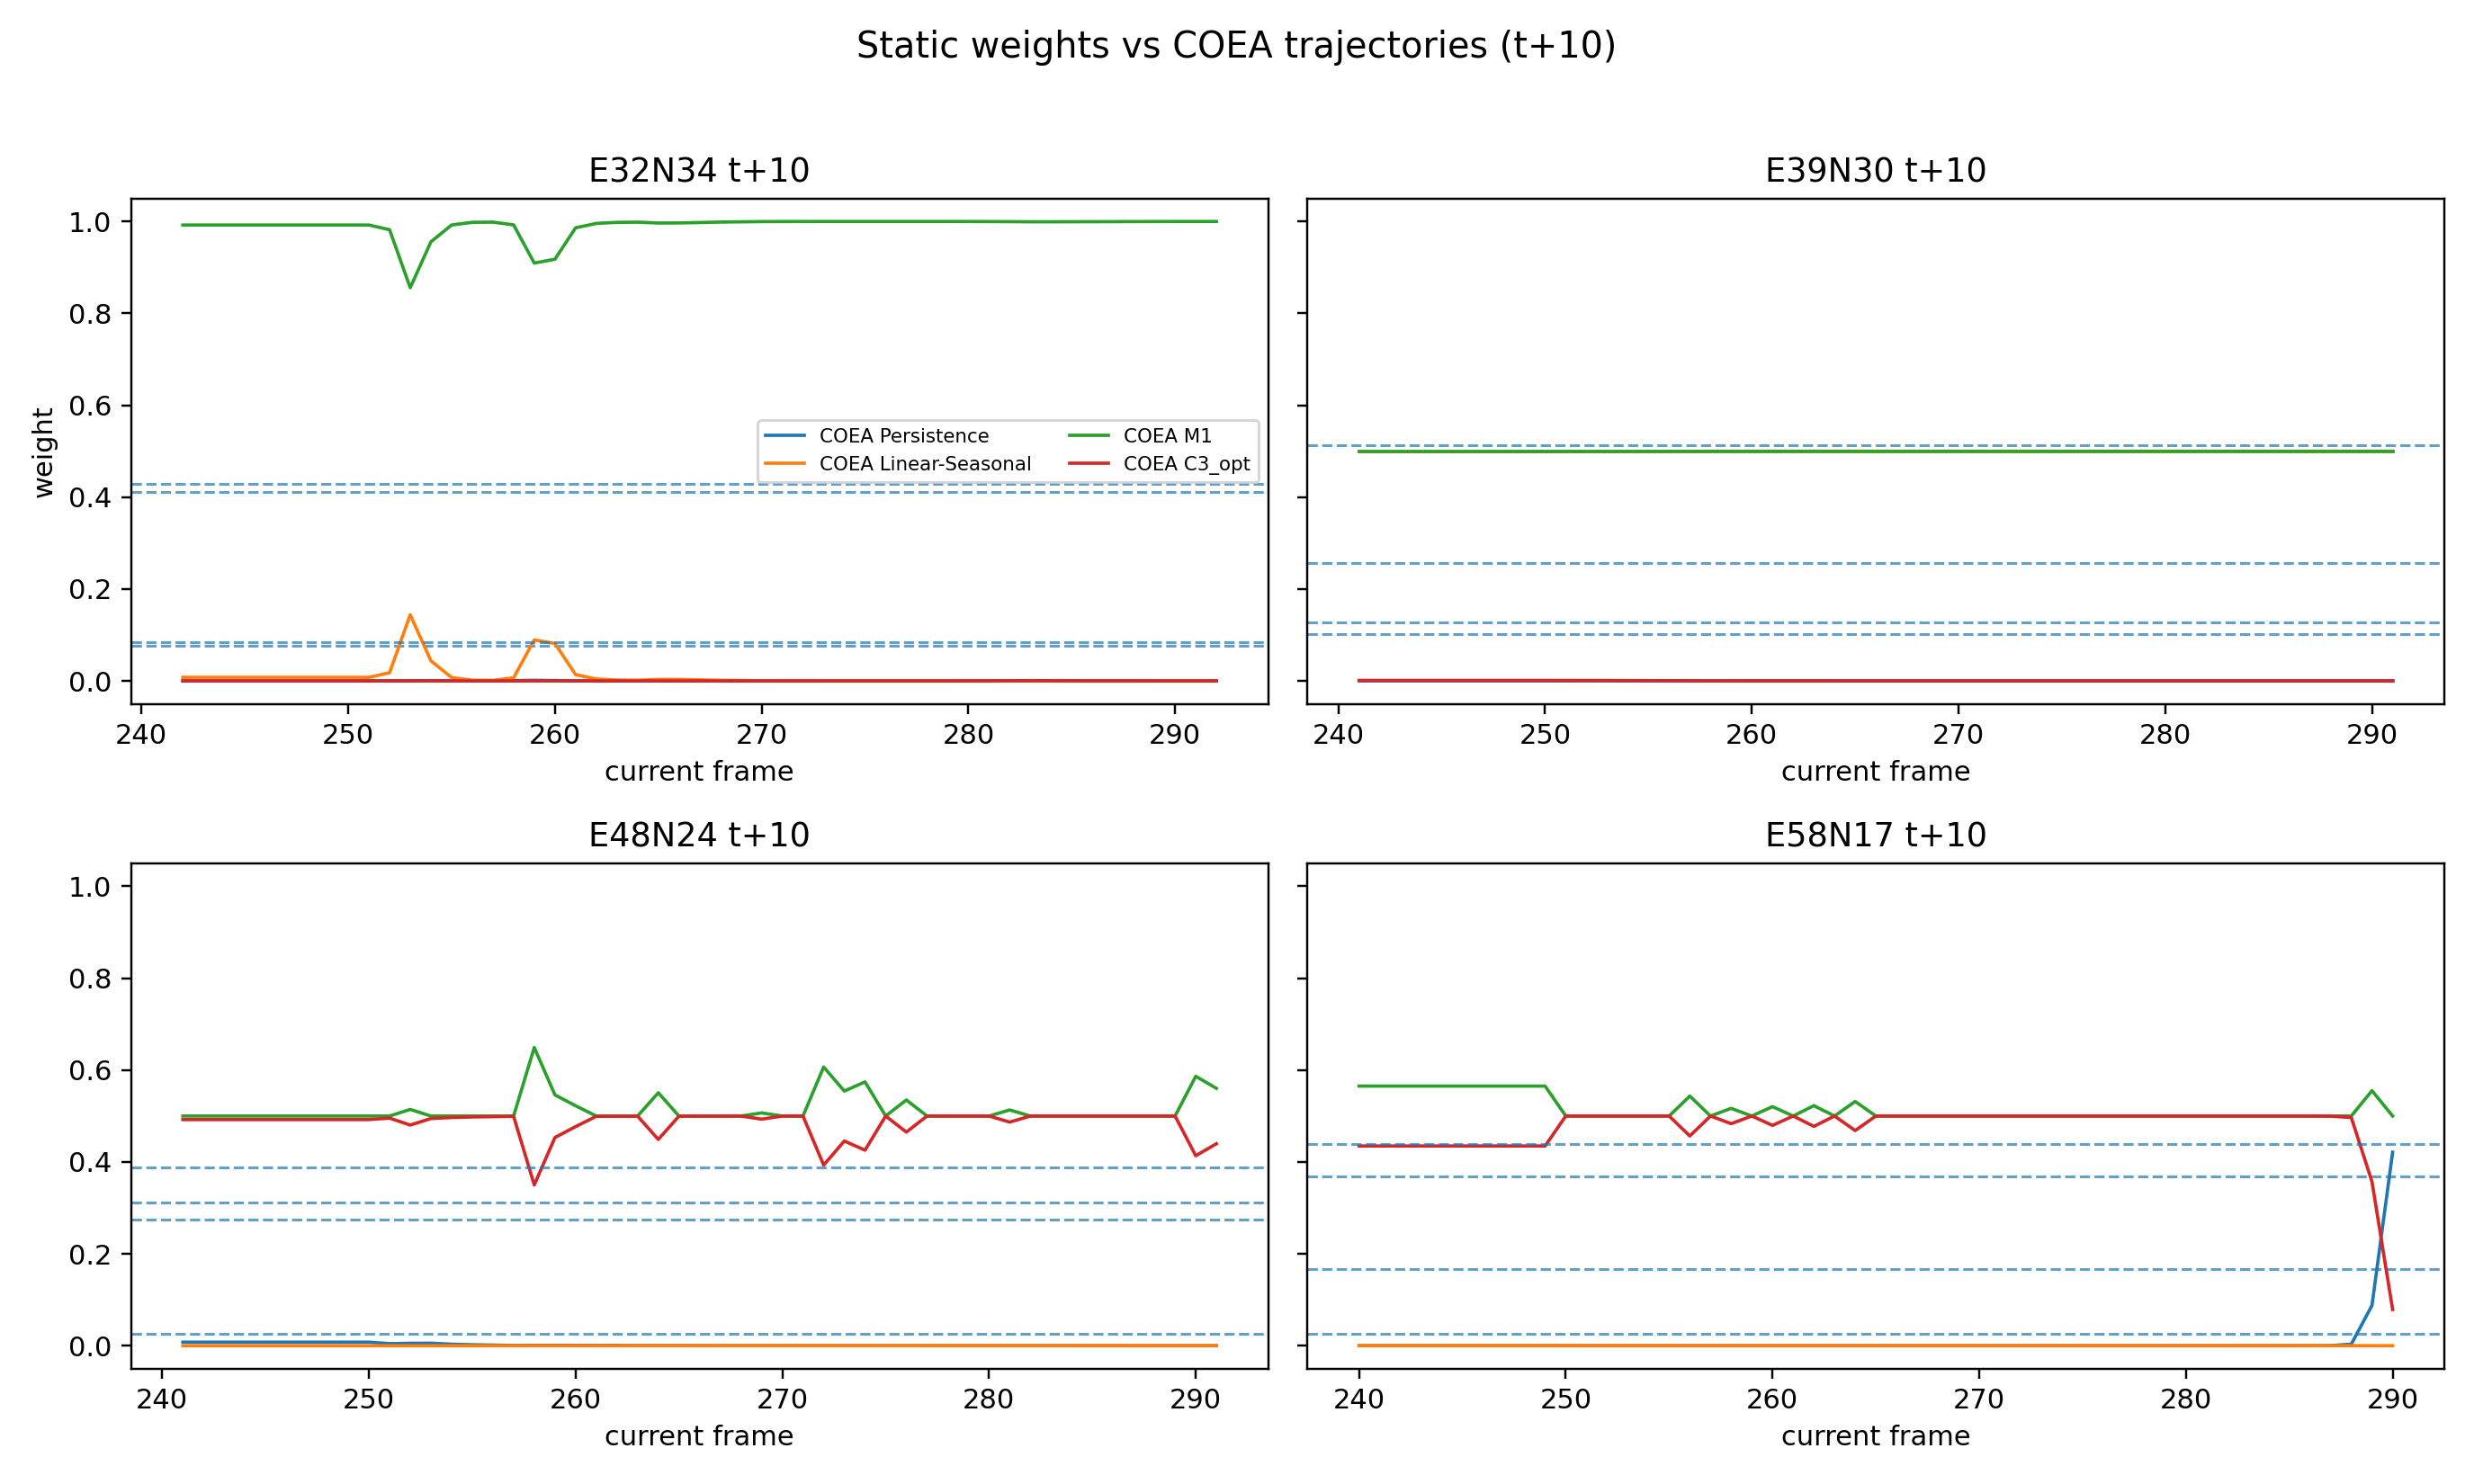
\includegraphics[width=0.98\textwidth]{figures/ready/fig_static_vs_coea_weight_drift.png}
  \caption{Weight drift from static VCEA to causal online aggregation (COEA). The drift pattern illustrates how delayed feedback and repeated online updates move the expert mixture away from the validation-calibrated optimum, which helps explain the performance gap between COEA and VCEA.}
  \label{fig:fig09}
\end{figure*}

\begin{figure*}[t]
  \centering
  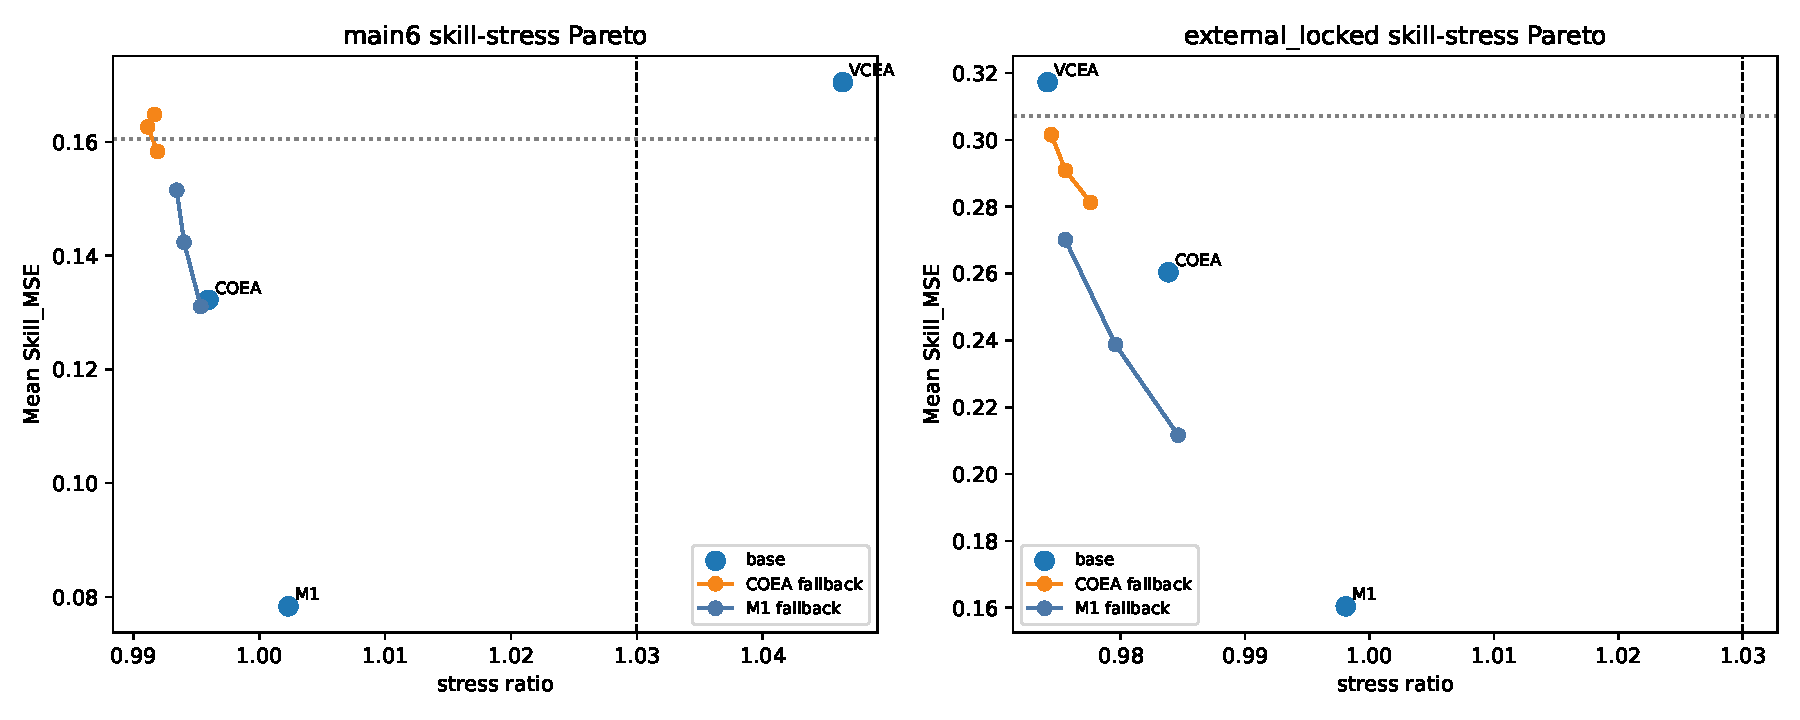
\includegraphics[width=0.98\textwidth]{figures/ready/fig_stress_skill_pareto.pdf}
  \caption{Skill--stress Pareto analysis for VCEA and SS-VCEA variants on the main-six and external locked settings. The selected SS-VCEA-COEA\_q97p5 variant sits close to the VCEA accuracy frontier while substantially reducing main-six stress risk.}
  \label{fig:fig10}
\end{figure*}

\begin{figure*}[t]
  \centering
  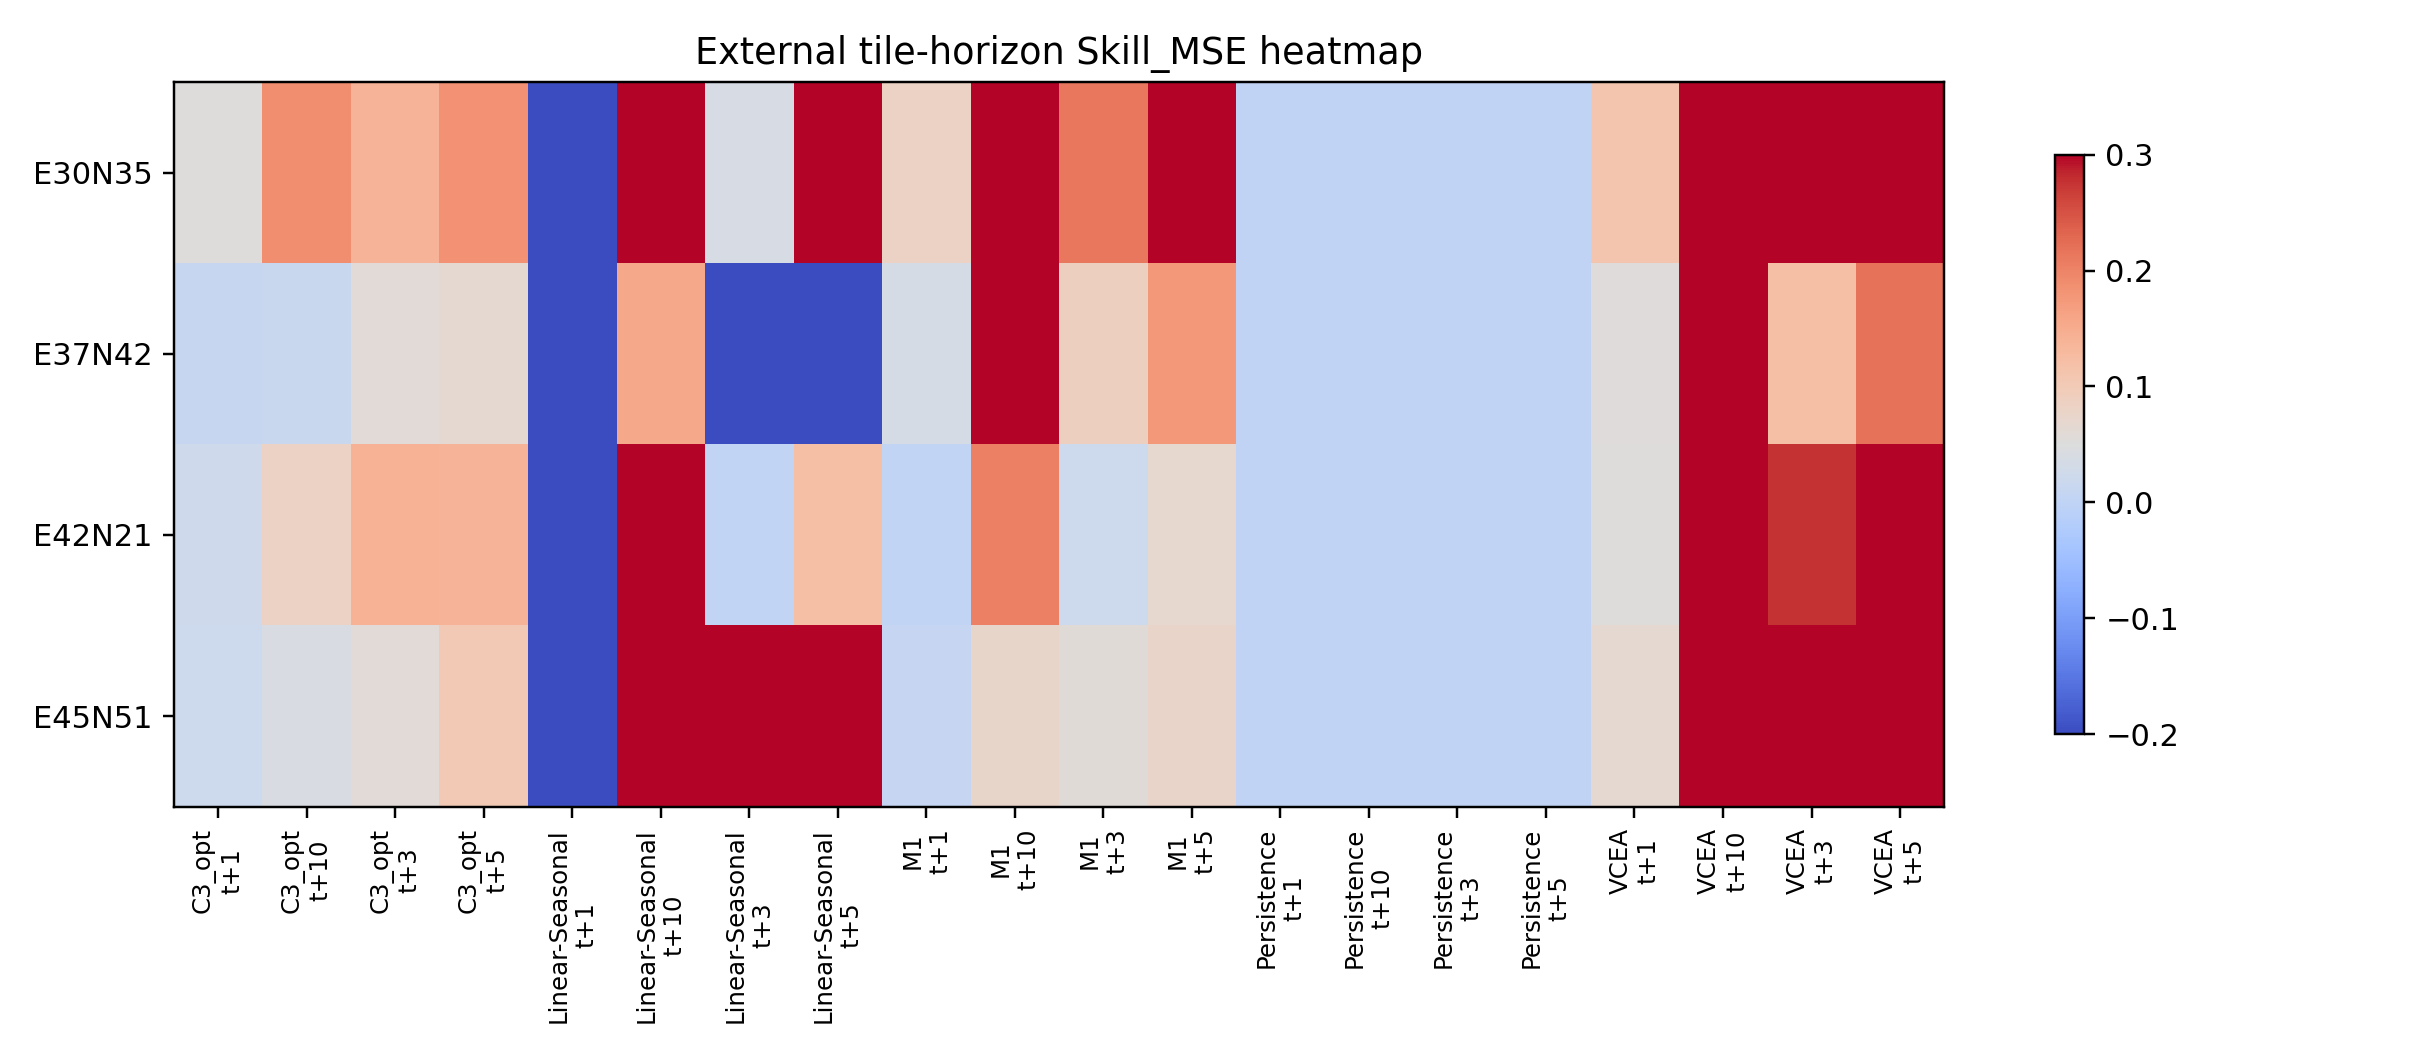
\includegraphics[width=0.98\textwidth]{figures/ready/fig_external_tile_generalization.png}
  \caption{External locked-evaluation results on four held-out tiles. VCEA retains positive Skill\_MSE under the frozen external protocol, and the selected SS-VCEA variant offers a conservative deployment alternative with limited accuracy loss.}
  \label{fig:fig11}
\end{figure*}

\begin{figure*}[t]
  \centering
  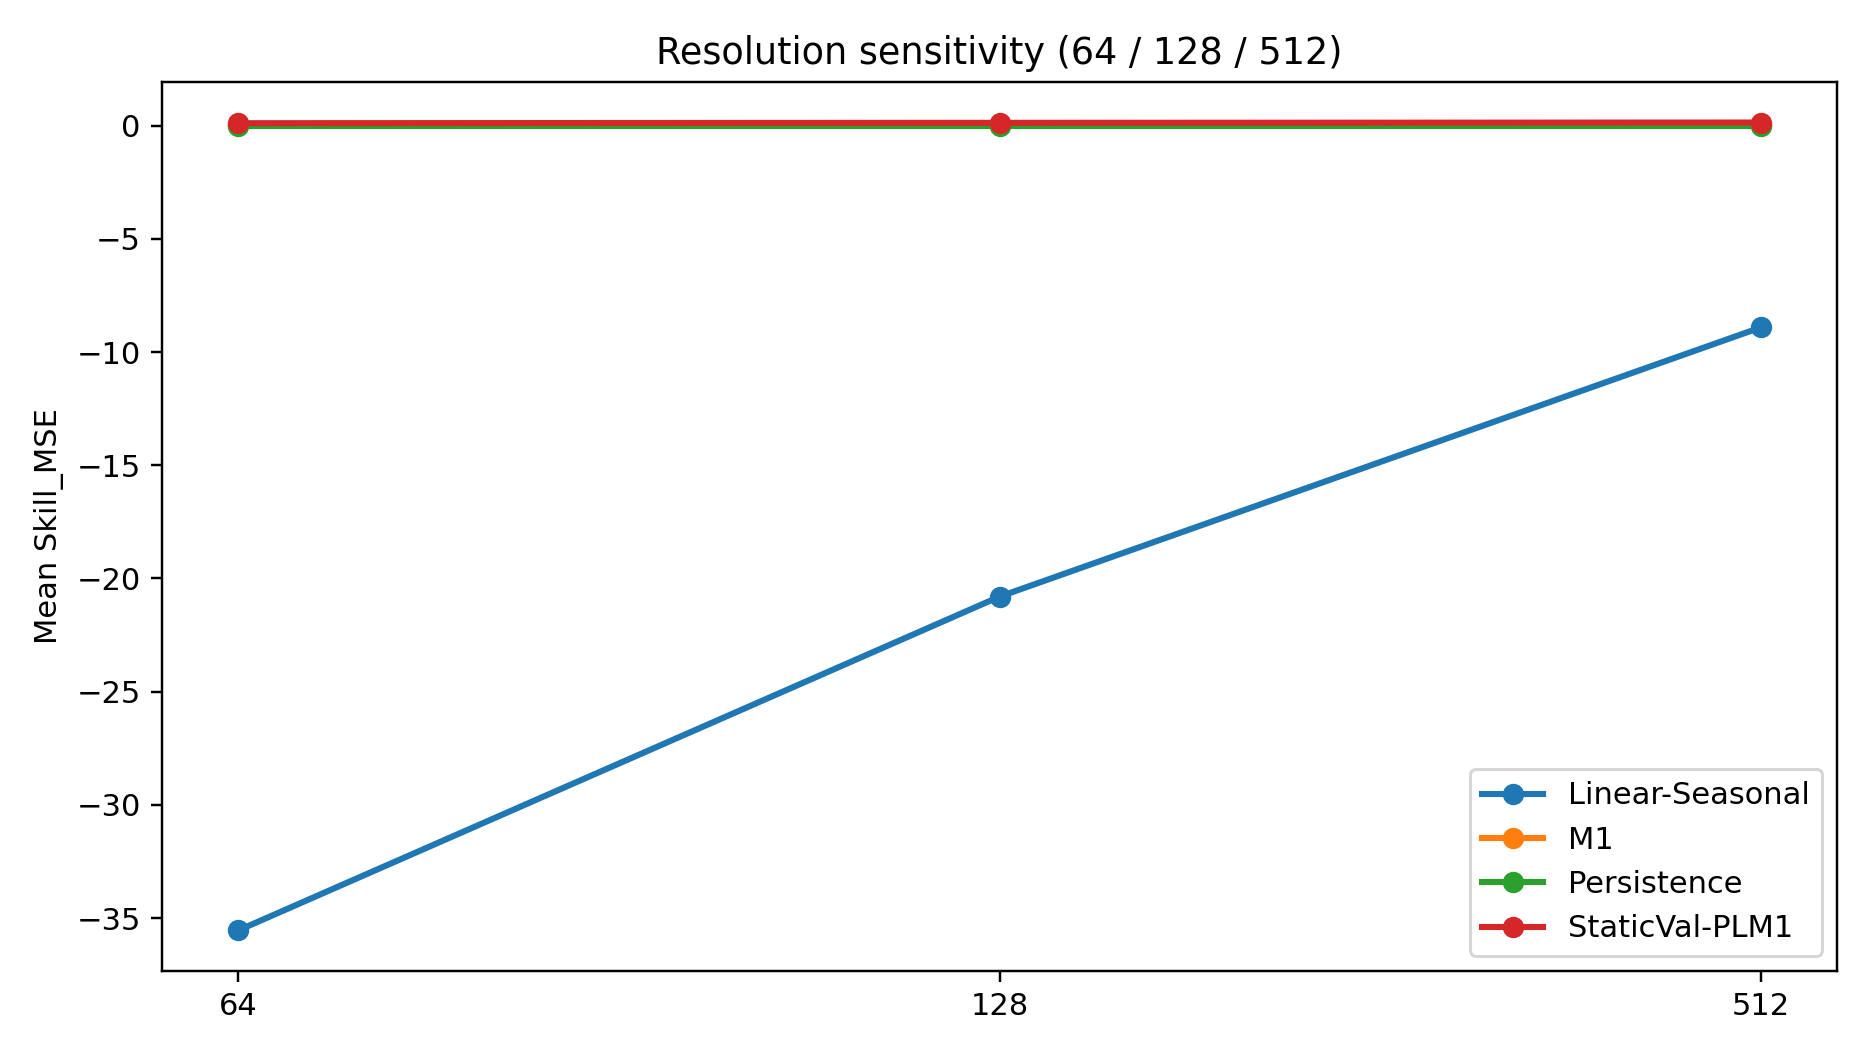
\includegraphics[width=0.98\textwidth]{figures/ready/fig_resolution_sensitivity.png}
  \caption{Resolution sensitivity of the model families. Single-model M1 degrades as the spatial grid increases from $64\times64$ to $512\times512$, whereas aggregation families continue to benefit from higher spatial resolution in sensitivity experiments.}
  \label{fig:fig12}
\end{figure*}

\begin{figure*}[t]
  \centering
  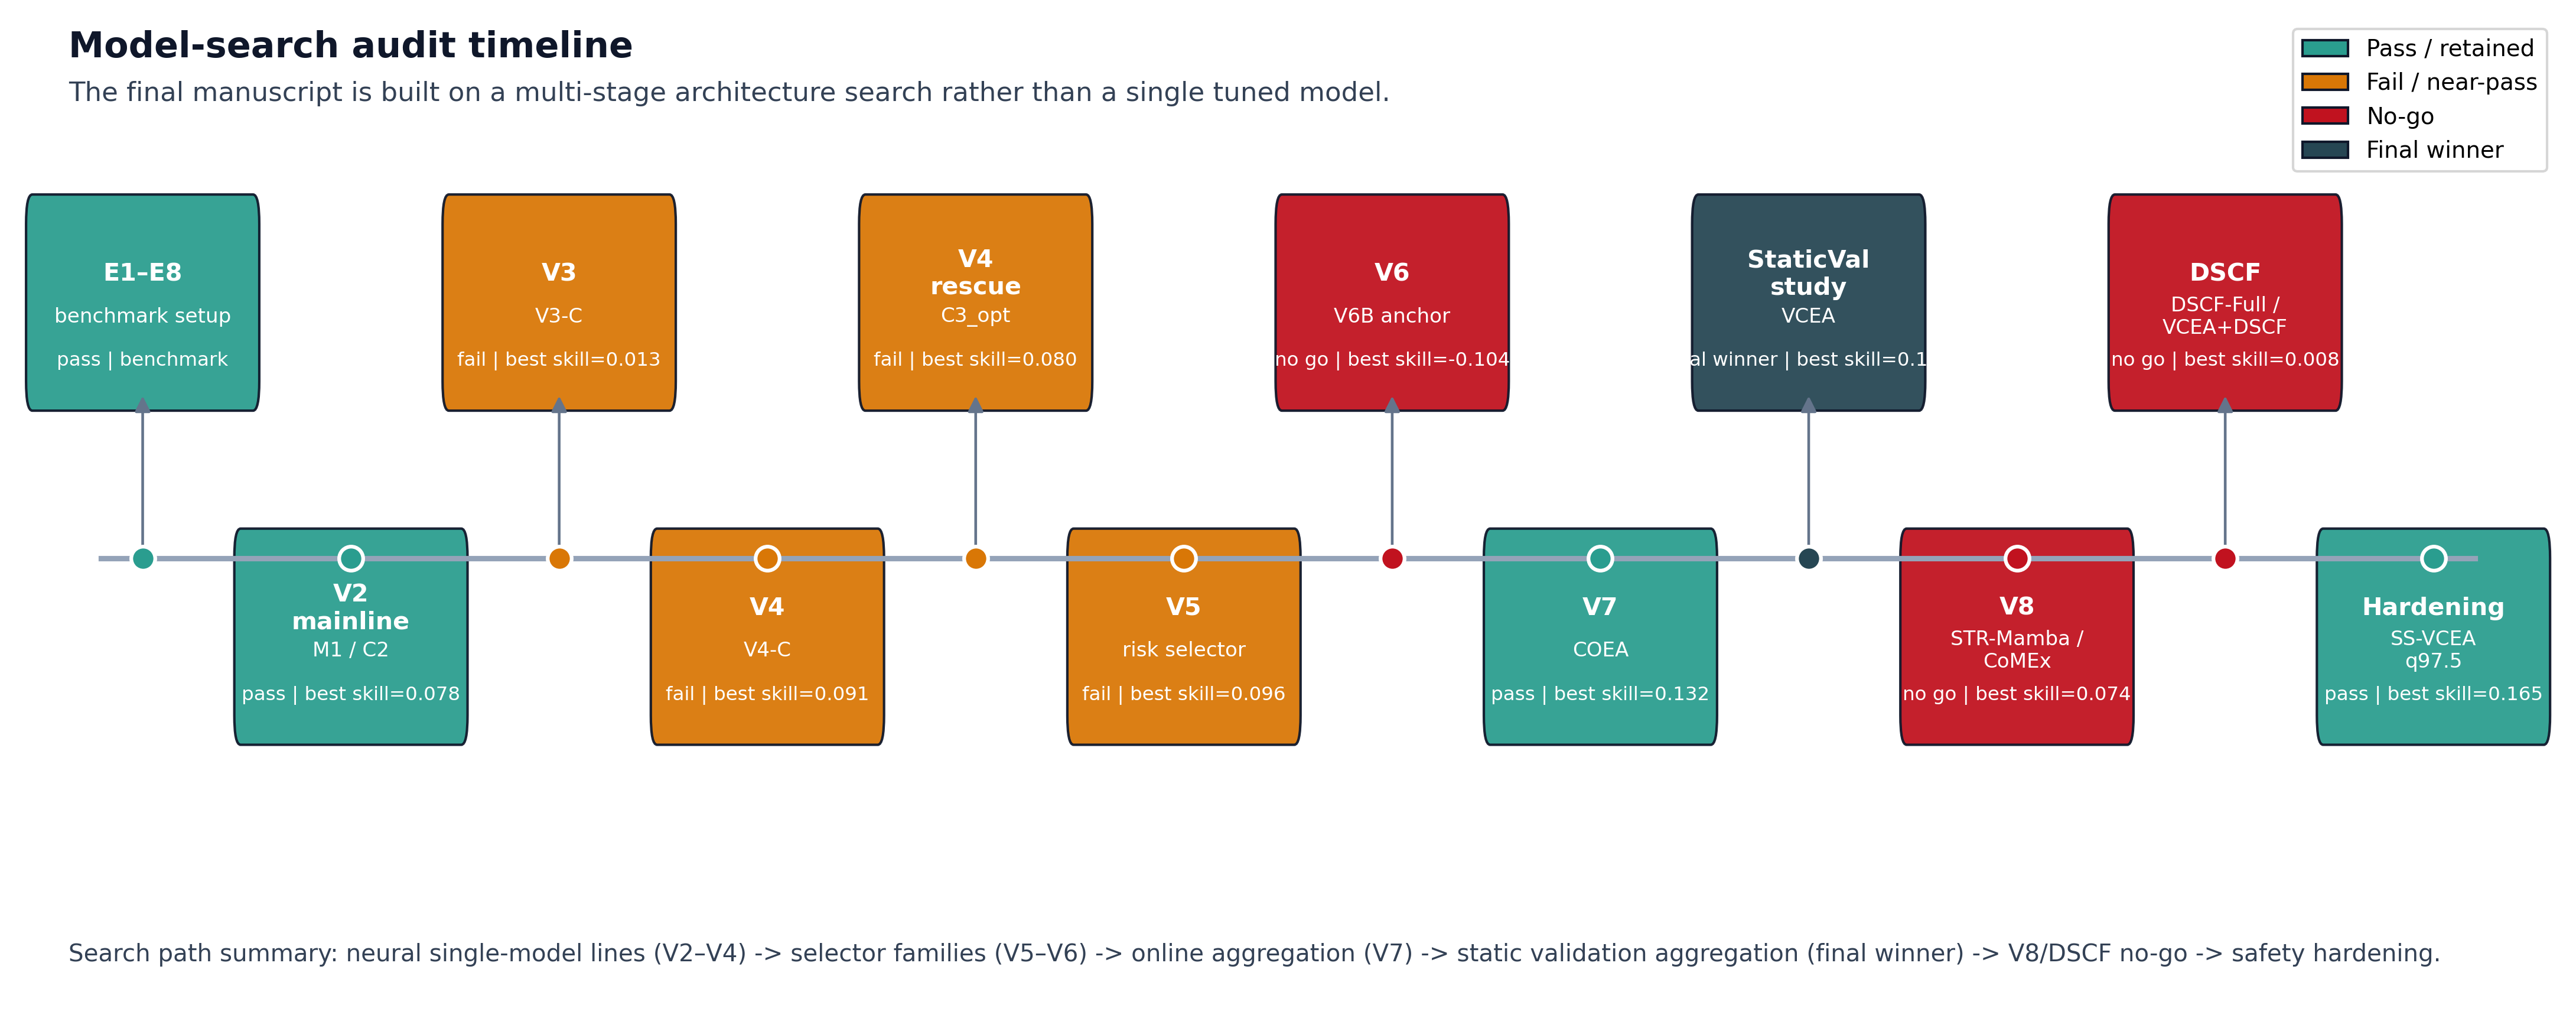
\includegraphics[width=0.98\textwidth]{figures/final/Fig13_model_search_audit_timeline.png}
  \caption{Model-search audit timeline from E1--E8 through V8 and DSCF hardening. The final manuscript is supported by a staged architecture search rather than a single tuned model: robust single-model baselines, selector families, online aggregation, static validation aggregation, and final safety hardening were all evaluated before freezing the mainline.}
  \label{fig:fig13}
\end{figure*}

\begin{figure*}[t]
  \centering
  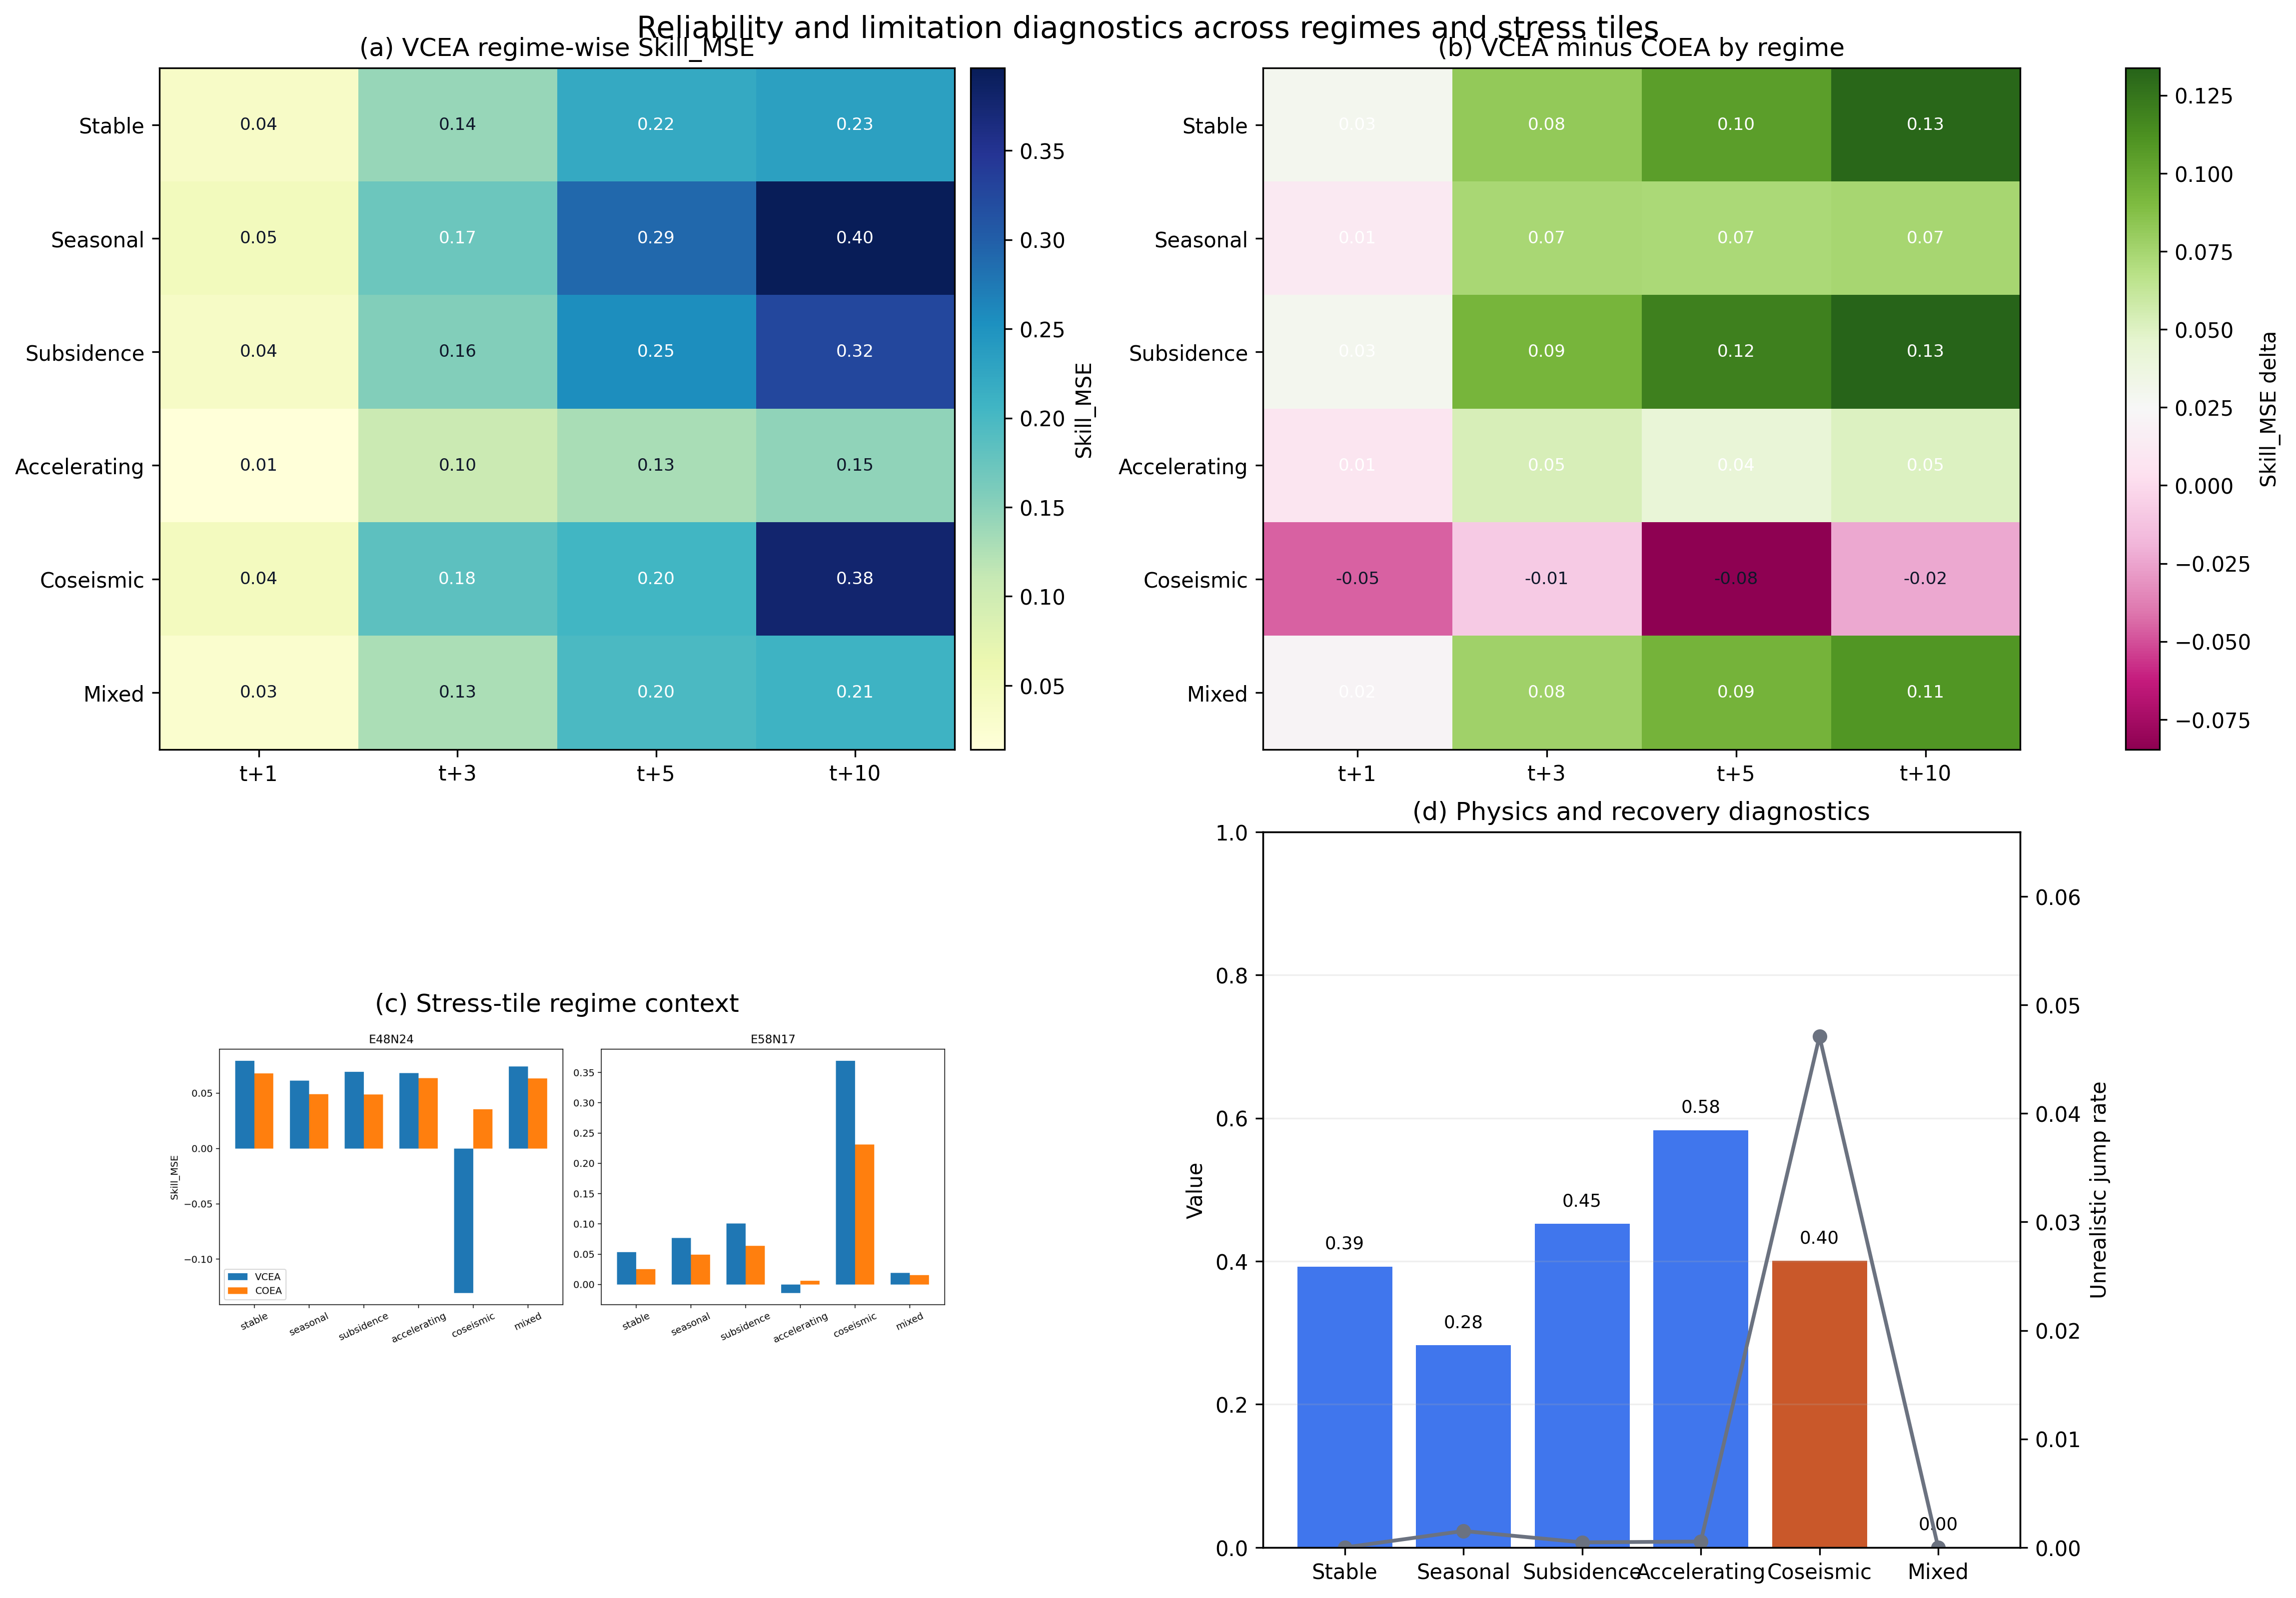
\includegraphics[width=0.98\textwidth]{figures/final/Fig14_physics_regime_diagnostic_panel.png}
  \caption{Reliability and limitation diagnostics across regimes and stress tiles. (a) Regime-wise Skill\_MSE of VCEA by horizon. (b) Regime-wise difference between VCEA and COEA. (c) Stress-tile regime context. (d) Physics-oriented diagnostics including sign consistency, post-event recovery ratio, and unrealistic jump behavior. These panels show that gains are not uniform across regimes and that coseismic cases remain the hardest operating condition.}
  \label{fig:fig14}
\end{figure*}

\subsection*{Tables}

\begin{table*}[t]
  \centering
  \caption{Metadata of the six main-development tiles and four external locked-evaluation tiles, including dominant regime labels, temporal span, valid-cell coverage, and raw point counts.}
  \label{tab:table01}
  \scriptsize
  % Embedded from tables/ready/Table01_tile_metadata_main_external.csv
  \begin{adjustbox}{max width=\textwidth}
  \begin{tabular}{lllp{0.13\textwidth}rrrr}
    \toprule
    Tile & Group & Role & \shortstack{Dominant\\regime} & Frames & Valid64 & Valid128 & \shortstack{Num\\points} \\
    \midrule
    E32N34 & main6 & source\_main & mixed & 303 & 0.772 & 0.698 & 138926 \\
    E32N35 & main6 & nearby\_seasonal & seasonal & 303 & 0.786 & 0.756 & 185125 \\
    E39N30 & main6 & subsidence\_1 & subsidence & 302 & 0.955 & 0.807 & 250830 \\
    E44N23 & main6 & subsidence\_2 & subsidence & 302 & 0.924 & 0.780 & 170553 \\
    E48N24 & main6 & coseismic\_1 & coseismic & 302 & 0.183 & 0.106 & 11911 \\
    E58N17 & main6 & coseismic\_2 & coseismic & 301 & 0.152 & 0.126 & 50260 \\
    E37N42 & external\_locked & external & mixed & 301 & 0.389 & 0.338 & 39626 \\
    E45N51 & external\_locked & external & mixed & 112 & 0.241 & 0.199 & 69604 \\
    E30N35 & external\_locked & external & mixed & 302 & 0.765 & 0.726 & 323481 \\
    E42N21 & external\_locked & external & mixed & 302 & 0.689 & 0.633 & 261823 \\
    \bottomrule
  \end{tabular}
  \end{adjustbox}
\end{table*}

\begin{table*}[t]
  \centering
  \caption{Unified data protocol used throughout the manuscript, including the EGMS product version, split strategy, input length, target horizons, primary and sensitivity resolutions, and descriptor policy.}
  \label{tab:table02}
  \footnotesize
  % Embedded from tables/ready/Table02_data_protocol.csv
  \begin{adjustbox}{max width=\textwidth}
  \begin{tabular}{p{0.18\textwidth}p{0.18\textwidth}p{0.52\textwidth}}
    \toprule
    \shortstack{Protocol\\item} & Setting & Note \\
    \midrule
    Product & EGMS 2019-2023 Ortho U & All formal results use the unified 2019-2023 Ortho U version. \\
    Main tiles & 6 & E32N34, E32N35, E39N30, E44N23, E48N24, E58N17. \\
    External locked tiles & 4 & E37N42, E45N51, E30N35, E42N21. \\
    Main split & 70/10/20 chronological & Leakage-safe train/val/test split. \\
    Input length & 16 frames & Unified for E1-E8 and all later mainline experiments. \\
    Horizons & t+1, t+3, t+5, t+10 & Multi-horizon nowcasting. \\
    Main resolution & 64$\times$64 & Primary regional nowcasting setting. \\
    Sensitivity resolutions & 128$\times$128, 512$\times$512 & Sensitivity/robustness only, not the main task. \\
    Descriptors & velocity, acceleration, seasonal amplitude, seasonal phase, residual std, trend R$^2$, DOY sin/cos & Fitted from train-window history only. \\
    Masking & valid-mask weighted metrics & Nearest-neighbor fill is for dense tensor construction only. \\
    Cross-site normalization & source-tile stats & Target descriptors still computed from target history. \\
    \bottomrule
  \end{tabular}
  \end{adjustbox}
\end{table*}

\begin{table*}[t]
  \centering
  \caption{Definitions of the primary accuracy, safety, robustness, diagnostic, and reproducibility metrics used in the study.}
  \label{tab:table03}
  \footnotesize
  % Embedded from tables/ready/Table03_metrics_definition.csv
  \begin{adjustbox}{max width=\textwidth}
  \begin{tabular}{p{0.14\textwidth}p{0.20\textwidth}p{0.56\textwidth}}
    \toprule
    \shortstack{Metric\\group} & Metric & Purpose \\
    \midrule
    Accuracy & RMSE & Primary magnitude error \\
    Accuracy & MAE & Robust average absolute error \\
    Accuracy & Skill\_MSE & 1 - MSE\_model / MSE\_persistence \\
    Accuracy & Skill\_RMSE & Relative RMSE improvement over persistence \\
    Accuracy & Acc@1mm / Acc@0.5mm & Thresholded accuracy \\
    Accuracy & SSIM & Structural similarity \\
    Safety & stress ratio & Worst-case risk / overcorrection safety measure \\
    Safety & fallback rate & Fraction of safe fallback in SS-VCEA \\
    Safety & correction magnitude & Magnitude of residual correction / risk \\
    Robustness & better tiles & How many tiles outperform the baseline \\
    Robustness & seed std & Stability across random seeds \\
    Robustness & external locked gain & Generalization beyond main-six \\
    Diagnostics & velocity-sign consistency & Sign consistency on moving pixels \\
    Diagnostics & jump rate & Unrealistic temporal jump frequency \\
    Diagnostics & post-event recovery ratio & Post-event stabilization diagnostic \\
    Diagnostics & regime-wise metrics & Stable/seasonal/subsidence/accelerating/coseismic/mixed diagnostics \\
    Efficiency/Repro & train time / inference time / peak memory & Engineering cost \\
    Efficiency/Repro & lineage / exact-proxy-transfer flags & Reproducibility provenance \\
    \bottomrule
  \end{tabular}
  \end{adjustbox}
\end{table*}

\begin{table*}[t]
  \centering
  \caption{Expert pool used by the aggregation family, including the persistence baseline, the linear-seasonal kinematic expert, the M1 neural expert, and the higher-capacity C3\_opt expert.}
  \label{tab:table04}
  \footnotesize
  % Embedded from tables/ready/Table04_expert_pool.csv
  \begin{adjustbox}{max width=\textwidth}
  \begin{tabular}{p{0.14\textwidth}p{0.16\textwidth}p{0.18\textwidth}p{0.42\textwidth}}
    \toprule
    Expert & Category & \shortstack{Training\\scope} & \shortstack{Role in\\pool} \\
    \midrule
    Persistence & strong baseline & No training & Short-horizon baseline and skill reference \\
    Linear-Seasonal & kinematic baseline & Per-tile fit & Trend + seasonal explicit expert \\
    M1 / C2 & neural expert & Full-six exact training & Best robust single-model expert with gated residual correction \\
    C3\_opt & state-space-inspired neural expert & Full-six exact training & Higher-capacity expert retained for complementarity \\
    \bottomrule
  \end{tabular}
  \end{adjustbox}
\end{table*}

\begin{table*}[t]
  \centering
  \caption{Protocol comparison between VCEA, COEA, and SS-VCEA, emphasizing weight source, update mode, safety mechanism, and whether any test-time tuning is allowed.}
  \label{tab:table05}
  \footnotesize
  % Embedded from tables/ready/Table05_aggregation_protocol_comparison.csv
  \begin{adjustbox}{max width=\textwidth}
  \begin{tabular}{p{0.10\textwidth}p{0.19\textwidth}p{0.16\textwidth}p{0.16\textwidth}cp{0.21\textwidth}}
    \toprule
    Method & \shortstack{Weight\\source} & \shortstack{Update\\mode} & \shortstack{Safety\\mechanism} & \shortstack{Test\\tuning} & Role \\
    \midrule
    VCEA & Validation-only static calibration & Tile$\times$horizon static weights & -- & No & Best-accuracy mainline \\
    COEA & Validation warm start + online update & Delayed-feedback online update & -- & No & Online aggregation baseline \\
    SS-VCEA & Reuse VCEA + validation-calibrated safety threshold & Static VCEA output & Risk-triggered hard fallback & No & Conservative deployment variant \\
    \bottomrule
  \end{tabular}
  \end{adjustbox}
\end{table*}

\begin{table*}[t]
  \centering
  \caption{Main-six comparison of the primary baselines, neural experts, and aggregation methods under the exact $64\times64$ setting.}
  \label{tab:table06}
  \scriptsize
  % Embedded from tables/ready/Table06_main_six_comparison.csv
  \begin{adjustbox}{max width=\textwidth}
  \begin{tabular}{llrrrrrp{0.22\textwidth}}
    \toprule
    Model & Category & \shortstack{Mean\\Skill\_MSE} & \shortstack{Gain\\vs M1} & \shortstack{Better tiles\\vs M1} & \shortstack{Stress\\ratio} & \shortstack{Mean Skill\\std} & Note \\
    \midrule
    VCEA & aggregation & 0.178 & 0.099 & 6 & 1.046 & 0.010 & main-six exact comparison \\
    SS-VCEA-COEA\_q97p5 & safe aggregation & 0.165 & 0.086 & 6 & 0.992 & 0.020 & selected conservative deployment variant \\
    COEA & aggregation & 0.132 & 0.054 & 6 & 0.996 & 0.021 & main-six exact comparison \\
    CRCF-COEA & aggregation & 0.127 & 0.049 & 6 & 1.002 & 0.022 & main-six exact comparison \\
    C3\_opt & neural expert & 0.080 & 0.001 & 2 & 0.992 & 0.020 & full-six near-pass expert \\
    M1 & baseline & 0.078 & -0.000 & 4 & 1.002 & 0.021 & main-six exact comparison \\
    Persistence & baseline & 0.000 & -0.078 & 0 & 1.000 & 0.000 & main-six exact comparison \\
    Linear-Seasonal & kinematic baseline & -36.149 & -36.228 & 0 & 16.845 & 0.000 & strong explicit kinematic baseline \\
    \bottomrule
  \end{tabular}
  \end{adjustbox}
\end{table*}

\begin{table*}[t]
  \centering
  \caption{VTSA summary metrics, including rank stability, top-$k$ retention, drift, and blocked-to-test robustness, which explain why validation-calibrated static aggregation remains effective.}
  \label{tab:table07}
  \footnotesize
  % Embedded from tables/ready/Table07_vtsa_summary.csv
  \begin{adjustbox}{max width=\textwidth}
  \begin{tabular}{p{0.22\textwidth}rp{0.54\textwidth}}
    \toprule
    VTSA metric & Value & Interpretation \\
    \midrule
    Mean Spearman & 0.778 & Validation-to-test expert ranking stability \\
    Mean Kendall & 0.731 & Rank consistency \\
    Top1 retention & 0.681 & Validation top-1 remains top-1 on test \\
    Top2 retention & 0.917 & Validation top-1 remains within test top-2 \\
    COEA mean L1 drift & 0.863 & Online weight drift relative to static weights \\
    Blocked-to-test skill & 0.173 & Static blocked validation robustness \\
    \bottomrule
  \end{tabular}
  \end{adjustbox}
\end{table*}

\begin{table*}[t]
  \centering
  \caption{Safety trade-off between VCEA and the selected SS-VCEA-COEA\_q97p5 variant on the main-six and external locked settings.}
  \label{tab:table08}
  \footnotesize
  % Embedded from tables/ready/Table08_vcea_vs_ssvcea_safety_tradeoff.csv
  \begin{adjustbox}{max width=\textwidth}
  \begin{tabular}{llrrrp{0.27\textwidth}}
    \toprule
    Model & Scope & \shortstack{Mean\\Skill\_MSE} & \shortstack{Stress\\ratio} & \shortstack{Gain/Loss\\vs VCEA} & Note \\
    \midrule
    VCEA & main-six & 0.171 & -- & -- & best-accuracy reference in hardening package \\
    SS-VCEA-COEA\_q97p5 & main-six & 0.165 & 0.992 & -0.006 & selected main-six safety trade-off \\
    VCEA & external\_locked & 0.317 & 0.974 & -- & frozen external exact evaluation \\
    SS-VCEA-COEA\_q97p5 & external\_locked & 0.302 & 0.974 & -0.016 & conservative deployment variant \\
    \bottomrule
  \end{tabular}
  \end{adjustbox}
\end{table*}

\begin{table*}[t]
  \centering
  \caption{Frozen external locked-evaluation summary, reporting the held-out performance of the candidate methods without any external-based retuning.}
  \label{tab:table09}
  \scriptsize
  % Embedded from tables/ready/Table09_external_locked_validation.csv
  \begin{adjustbox}{max width=\textwidth}
  \begin{tabular}{lrrrrrrr}
    \toprule
    Model & \shortstack{Skill\_MSE\\mean} & \shortstack{Skill\_MSE\\std} & \shortstack{RMSE\\[mm] mean} & \shortstack{Acc@1mm\\[%] mean} & SSIM mean & \shortstack{Worst RMSE/\\persistence} & \shortstack{Gain/Loss\\vs VCEA} \\
    \midrule
    VCEA & 0.317 & 0.003 & 0.611 & 92.339 & 0.942 & 0.974 & 0.000 \\
    SS-VCEA-COEA\_q97p5 & 0.302 & 0.003 & -- & -- & -- & 0.974 & -0.016 \\
    M1 & 0.160 & 0.005 & 0.697 & 89.288 & 0.929 & 0.998 & -0.157 \\
    C3\_opt & 0.083 & 0.013 & 0.753 & 87.329 & 0.925 & 0.994 & -0.235 \\
    Persistence & 0.000 & 0.000 & 0.790 & 86.586 & 0.927 & 1.000 & -0.317 \\
    Linear-Seasonal & -0.788 & 0.000 & 0.791 & 87.434 & 0.926 & 2.966 & -1.105 \\
    \bottomrule
  \end{tabular}
  \end{adjustbox}
\end{table*}

\begin{table*}[t]
  \centering
  \caption{Resolution sensitivity across model families and aggregation types, covering the primary $64\times64$ setting and the $128\times128$ and $512\times512$ sensitivity analyses.}
  \label{tab:table10}
  \scriptsize
  % Embedded from tables/ready/Table10_resolution_sensitivity.csv
  \begin{adjustbox}{max width=\textwidth}
  \begin{tabular}{lrrrrr}
    \toprule
    Model & Resolution & \shortstack{Mean\\Skill\_MSE} & Mean RMSE [mm] & \shortstack{Stress\\ratio} & \shortstack{Better tiles\\vs M1} \\
    \midrule
    VCEA\_exact & 64 & 0.150 & 0.866 & 1.046 & 2 \\
    COEA\_exact & 64 & 0.129 & 0.877 & 0.997 & 3 \\
    C3\_opt & 64 & 0.084 & 0.905 & 1.011 & 2 \\
    M1 & 64 & 0.047 & 0.924 & 1.002 & 3 \\
    M0 & 64 & 0.016 & 0.936 & 1.049 & 0 \\
    Persistence & 64 & 0.000 & 0.951 & 1.000 & 0 \\
    Linear-Seasonal & 64 & -35.548 & 4.307 & 13.892 & 0 \\
    VCEA\_exact & 128 & 0.173 & 1.230 & 1.014 & 3 \\
    COEA\_exact & 128 & 0.134 & 1.261 & 0.999 & 3 \\
    C3\_opt & 128 & 0.085 & 1.295 & 1.091 & 2 \\
    M1 & 128 & 0.028 & 1.347 & 1.001 & 3 \\
    M0 & 128 & 0.016 & 1.355 & 1.012 & 0 \\
    Persistence & 128 & 0.000 & 1.371 & 1.000 & 0 \\
    Linear-Seasonal & 128 & -20.803 & 4.754 & 10.488 & 0 \\
    VCEA\_exact & 512 & 0.189 & 1.736 & 0.990 & 3 \\
    COEA\_exact & 512 & 0.145 & 1.783 & 0.999 & 3 \\
    C3\_opt & 512 & 0.116 & 1.814 & 1.054 & 3 \\
    M1 & 512 & 0.015 & 1.934 & 1.000 & 3 \\
    Persistence & 512 & 0.000 & 1.952 & 1.000 & 0 \\
    M0 & 512 & -0.010 & 1.959 & 1.032 & 0 \\
    Linear-Seasonal & 512 & -8.910 & 4.897 & 6.762 & 0 \\
    \bottomrule
  \end{tabular}
  \end{adjustbox}
\end{table*}

\begin{table*}[t]
  \centering
  \caption{Architecture-search audit table summarizing the strongest candidate, best Skill\_MSE, verdict, and reason for retention or rejection at each major search stage.}
  \label{tab:table11}
  \scriptsize
  % Embedded from tables/ready/Table11_architecture_search_audit.csv
  \begin{adjustbox}{max width=\textwidth}
  \begin{tabular}{p{0.11\textwidth}p{0.15\textwidth}rrp{0.46\textwidth}}
    \toprule
    Stage & Best candidate & \shortstack{Best mean\\Skill\_MSE} & Verdict & \shortstack{Reason not final\\or role} \\
    \midrule
    V2 mainline & M1 / C2 PG-RQ-ACT & 0.078 & pass & Best robust single-model line; kept as neural expert/baseline \\
    V3 & V3-C quick & 0.013 & fail & Too weak versus M1 despite acceptable complexity \\
    V4 & V4-C original & 0.091 & fail & Accuracy-credible but compute-no-go \\
    V4 rescue & C3\_opt & 0.080 & fail & Runtime fixed but full-six generalization insufficient \\
    V5 & risk-aware selector & 0.096 & fail & Oracle space exists but learned selector under-delivers on full-six \\
    V6 & V6B\_anchor\_risk\_l20 & -0.104 & no\_go & Anchored soft selector unstable and stress-unsafe \\
    V7 & COEA audited & 0.132 & pass & First successful aggregation family beyond M1 \\
    StaticVal study & VCEA & 0.178 & final\_winner & Best overall accuracy trade-off \\
    V8 & STR-Mamba / CoMEx & 0.074 & no\_go & New architectures did not beat VCEA mainline \\
    DSCF & DSCF-Full / VCEA+DSCF & 0.008 & no\_go & Task-native consistency direction did not pass quick gate \\
    \bottomrule
  \end{tabular}
  \end{adjustbox}
\end{table*}

\begin{table*}[t]
  \centering
  \caption{Reproducibility package and provenance map, listing the manifests, split definitions, cache registries, and claim-to-result tracing artifacts that support the final manuscript.}
  \label{tab:table12}
  \scriptsize
  % Embedded from tables/ready/Table12_reproducibility_package.csv
  \begin{adjustbox}{max width=\textwidth}
  \begin{tabular}{p{0.16\textwidth}p{0.48\textwidth}p{0.25\textwidth}}
    \toprule
    Artifact & Path & Role \\
    \midrule
    Product manifest & \path{data/manifests/product_manifest.csv} & Data product provenance \\
    Tile manifest & \path{data/manifests/tile_manifest.csv} & Main/external tile provenance \\
    Resolution manifest & \path{data/manifests/resolution_manifest.csv} & 64/128/512 scope freeze \\
    Main split & \path{splits/main6_train_val_test.json} & Formal main-six split \\
    External locked split & \path{splits/external4_locked_eval.json} & Frozen external evaluation \\
    Expert cache registry & \path{cache/expert_cache_registry.yaml} & Expert prediction cache provenance \\
    Aggregation weight registry & \path{cache/aggregation_weight_registry.yaml} & Aggregation calibration provenance \\
    Lineage table & \path{outputs/tgrs_2019_2023/hardening_package/reproducibility/result_lineage_table.csv} & Experiment-to-artifact mapping \\
    Claim-to-result map & \path{outputs/tgrs_2019_2023/hardening_package/reproducibility/claim_to_result_map.md} & Claim audit \\
    Paper table source map & \path{outputs/tgrs_2019_2023/hardening_package/reproducibility/paper_table_source_map.csv} & Table-to-source provenance \\
    Figure source map & \path{outputs/tgrs_2019_2023/hardening_package/reproducibility/figure_source_map.csv} & Figure-to-source provenance \\
    Exact/proxy/transfer flags & \path{outputs/tgrs_2019_2023/hardening_package/reproducibility/exact_proxy_transfer_flags.csv} & Historical artifact status \\
    \bottomrule
  \end{tabular}
  \end{adjustbox}
\end{table*}

\subsection*{Figure and Table Ordering Notes}
\begin{itemize}
  \item Figures 1--4 define the benchmark, leakage-safe protocol, baseline difficulty, and method overview.
  \item Figures 5--10 cover mechanism, main results, ranking stability, drift, and the safety trade-off.
  \item Figures 11--14 cover external robustness, resolution sensitivity, model-search audit, and reliability diagnostics.
  \item Tables 1--5 define data, metrics, experts, and protocols; Tables 6--12 summarize results, safety, robustness, and reproducibility.
\end{itemize}
